\section{Efficiency}
\label{sec:efficiency}

Lastly, we are interested in estimating the efficiency of the detectors.
The efficiency is the number of events detected over the number of photons emitted by the source. This parameter is extremely important for the correct characterization of the detectors, and in the following subsections are listed different methods used to get this estimation.

\subsection{First Estimate}
\label{sub:rough}

\begin{comment}
\begin{figure}[H]
    \centering
    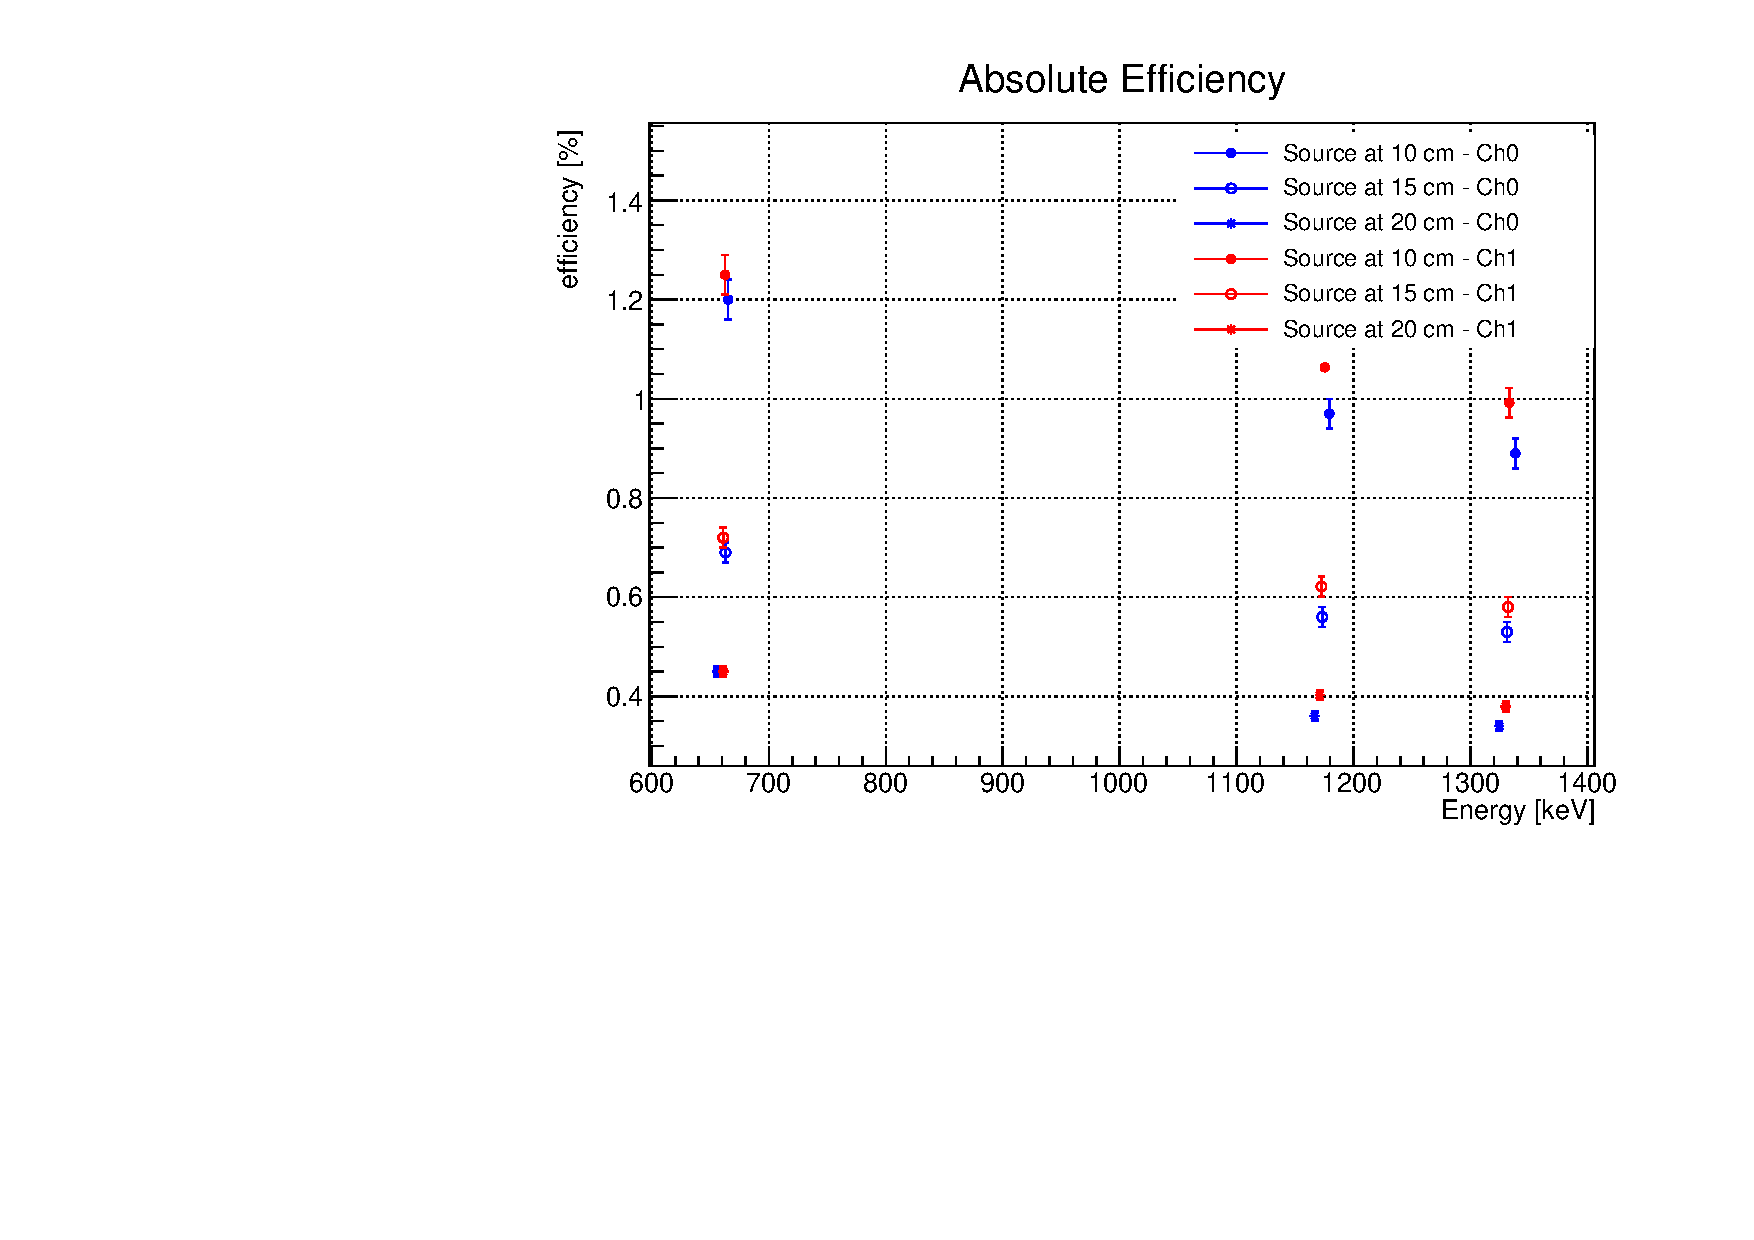
\includegraphics[scale=0.5]{Images/analysis/efficiency/eff_rough.pdf}
    \caption{First rough estimate of the absolute efficiency of the detectors, with detector 0 in blue and detector 1 in red, for each distance.}
    \label{fig:eff_rough}
\end{figure}
\end{comment}

\begin{figure}[H]
	\begin{minipage}[c]{0.35\linewidth}
    \centering
	\subfloat[][Sources at 10 cm.]{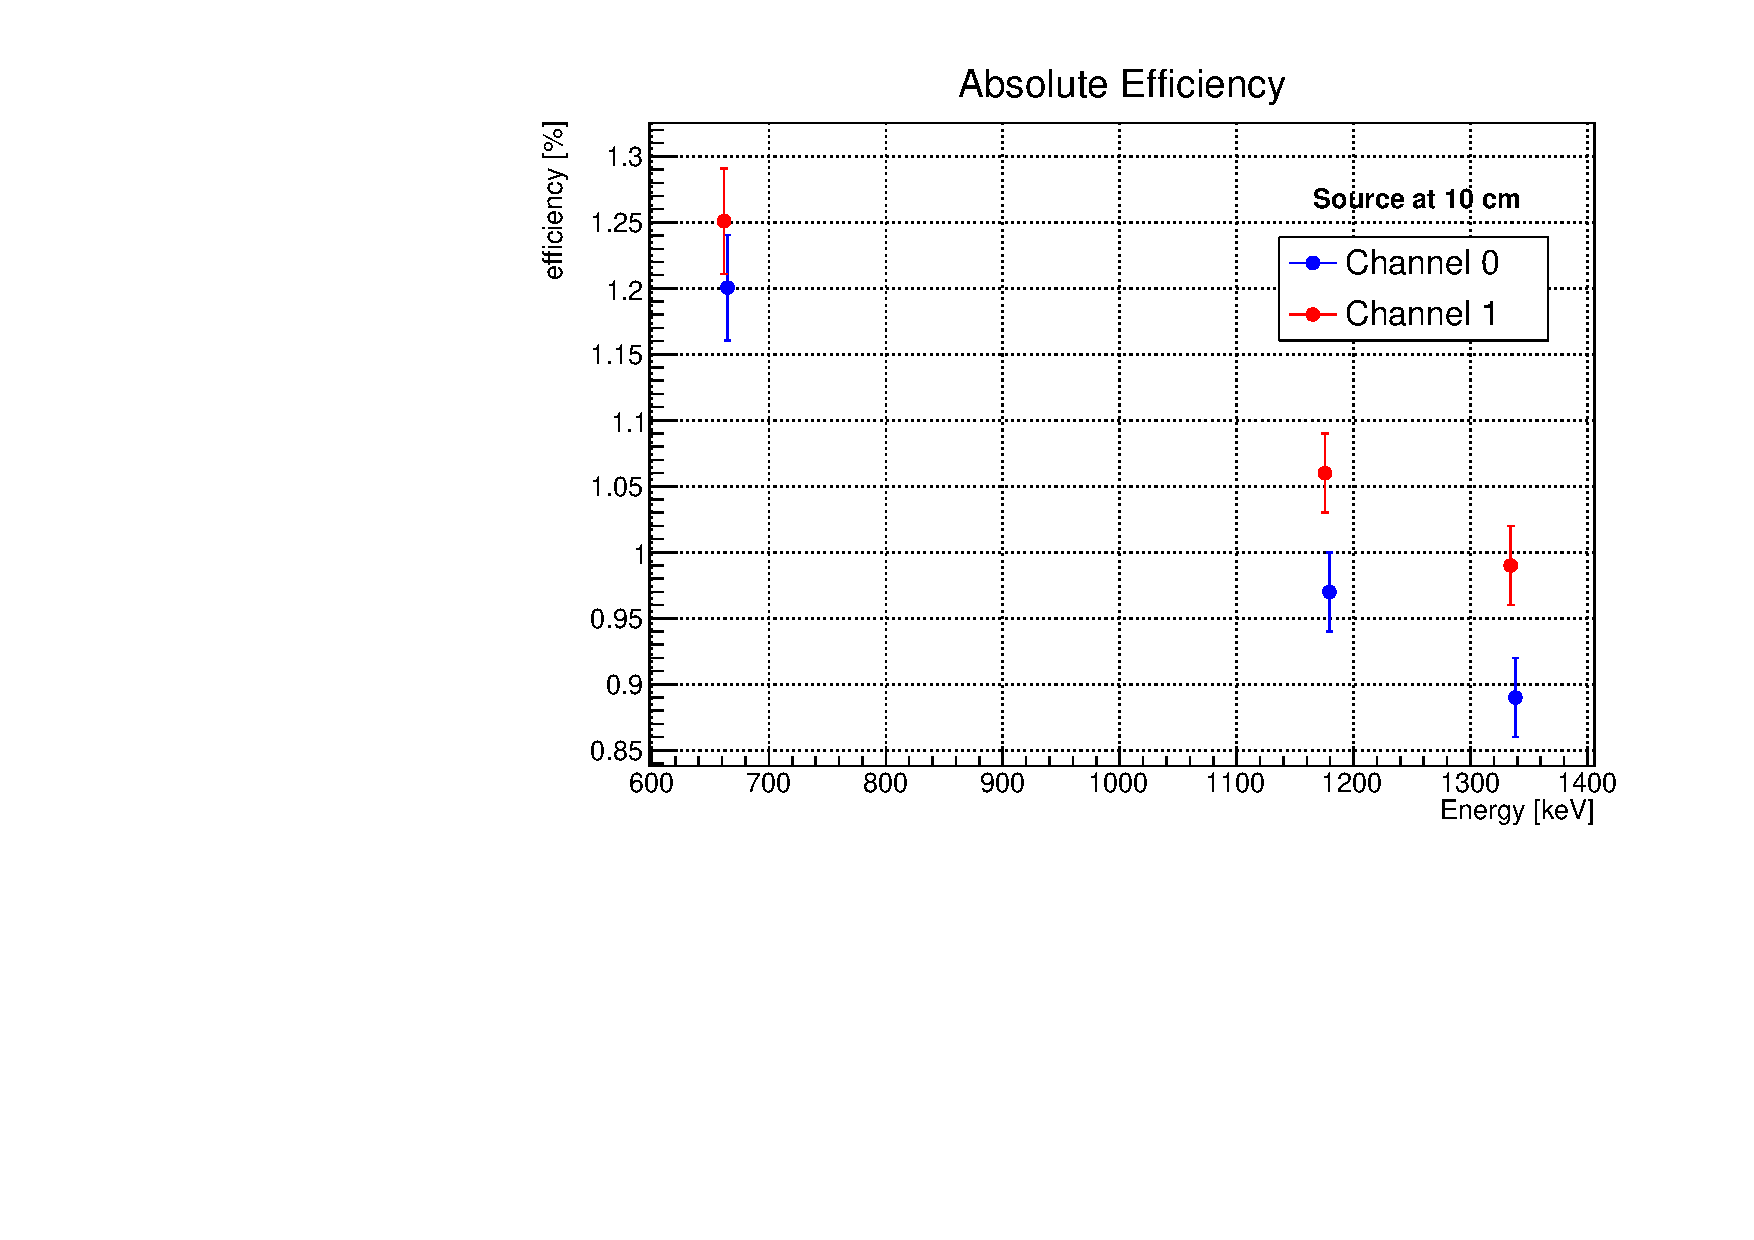
\includegraphics[width=0.95\textwidth]{Images/analysis/efficiency/eff_rough_10.pdf} \label{fig:rough_10} }
	\end{minipage}
	\begin{minipage}[]{0.35\linewidth}
	\centering
	\subfloat[][Sources at 15 cm.]{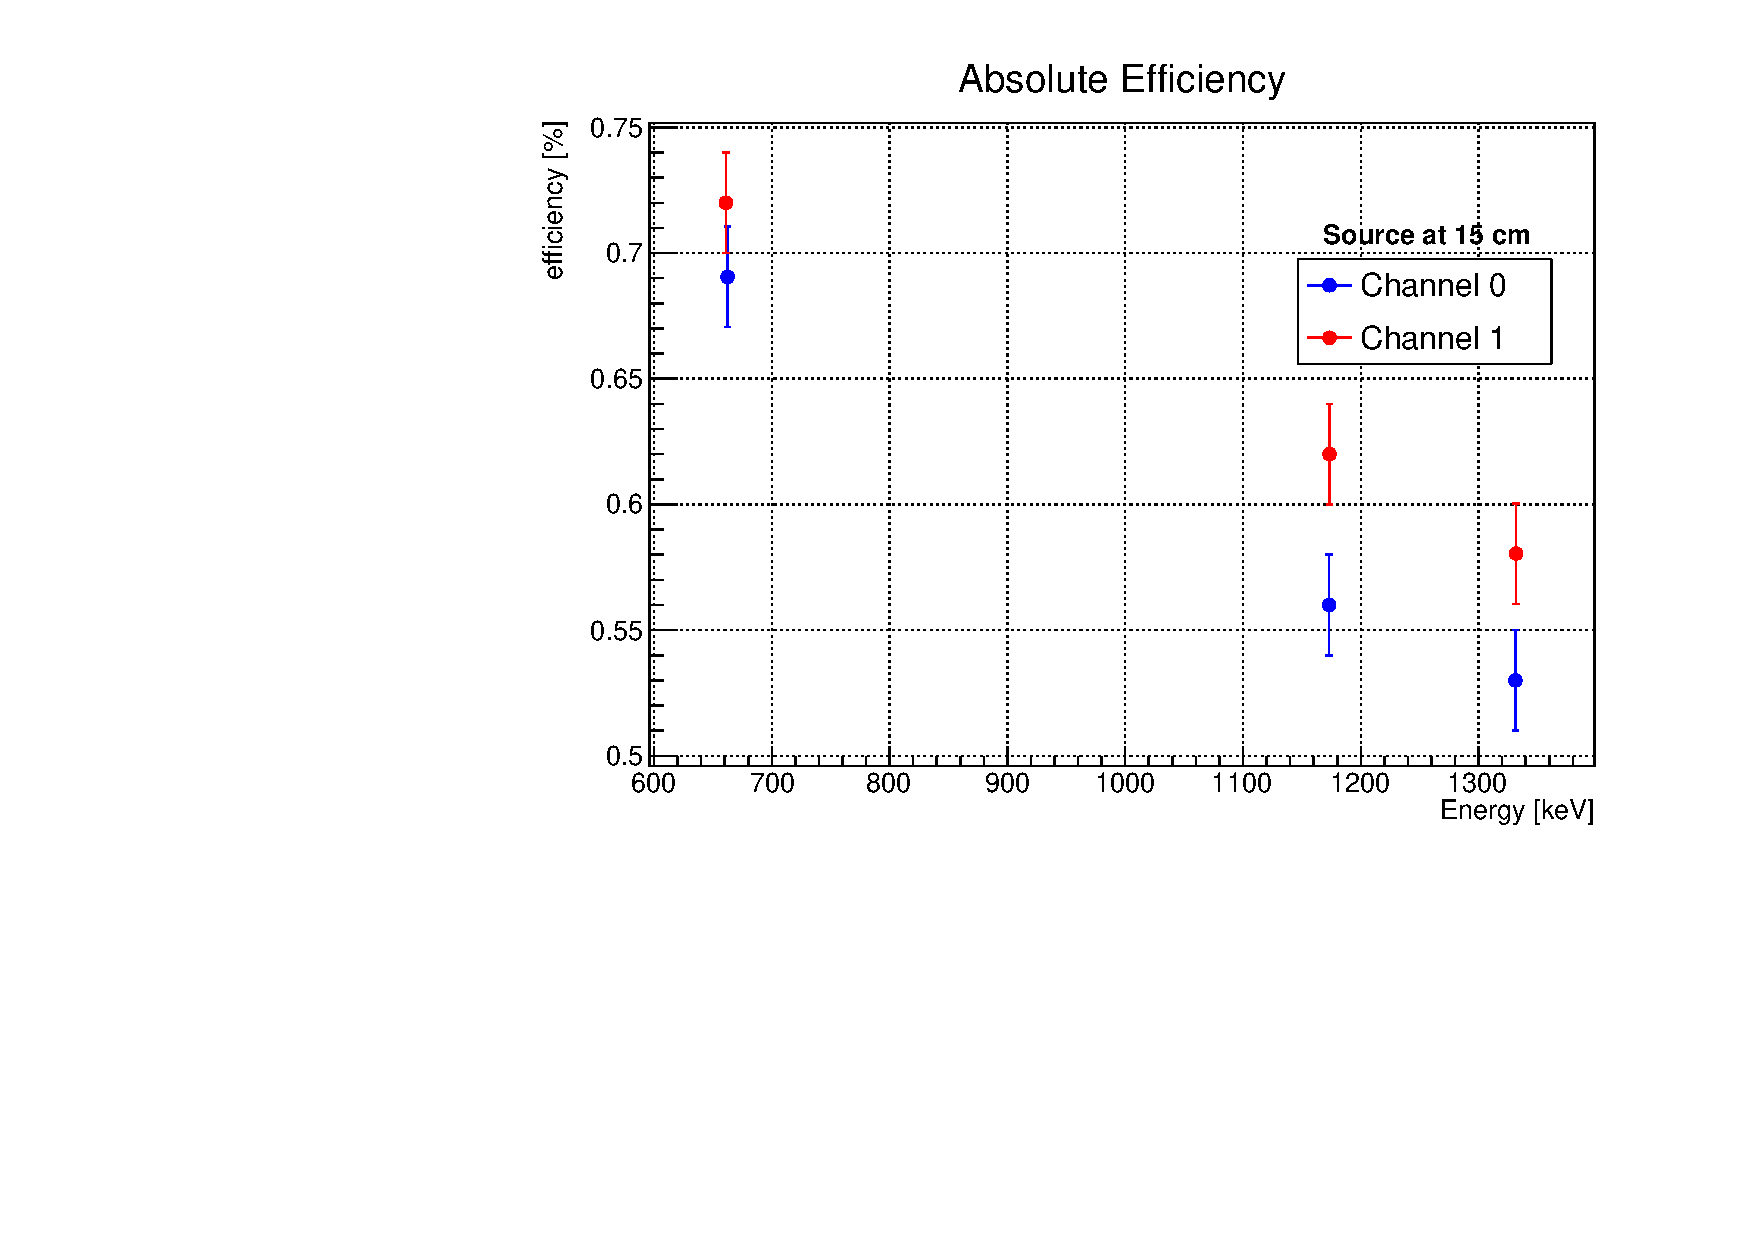
\includegraphics[width=0.95\textwidth]{Images/analysis/efficiency/eff_rough_15.pdf}  \label{fig:rough_15} }
	\end{minipage}
    \begin{minipage}[c]{0.35\linewidth}
    \centering
	\subfloat[][Source at 20 cm]{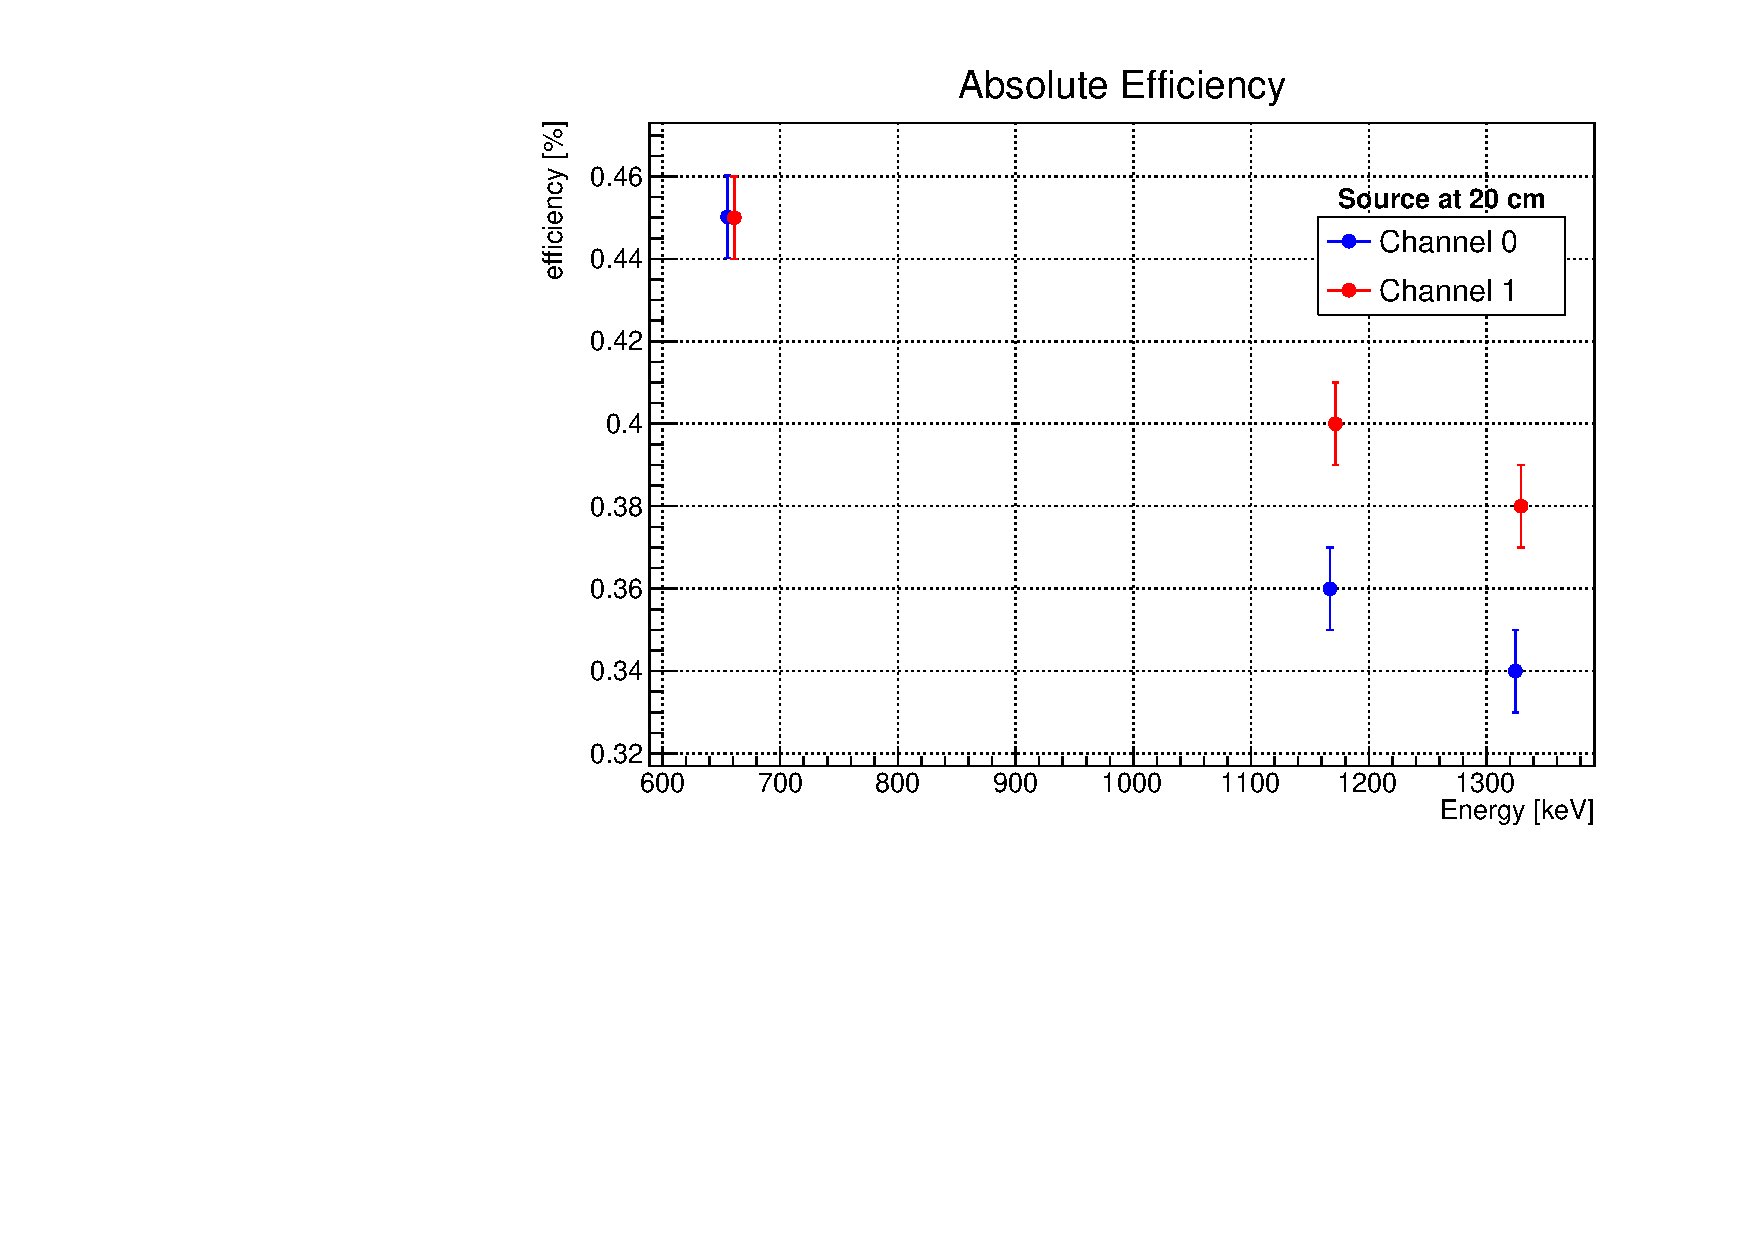
\includegraphics[width=0.95\textwidth]{Images/analysis/efficiency/eff_rough_20.pdf} \label{fig:rough_20} }
	\end{minipage}
	\caption{First rough estimate of the absolute efficiency of the detectors, with detector 0 in blue and detector 1 in red, for each distance.}
    \label{fig:eff_rough}
	\end{figure}
 
To make a first rough estimate of the efficiency, we take the peaks of $^{137}$Cs and $^{60}$Co, and compute the area subtended by the gaussian without the background, which corresponds to the number of events detected at each energy. For this first estimation, we also considere the events in the peak of 2505 keV for $^{60}$Co. This peak, as said before, corresponds to the detection of the two gammas of 1172 keV and 1332 keV from the same detector, that collects them as one event. Since the presence of this peak means that a gamma of 1172 keV, as well as a gamma of 1332 keV, are detected, we estimate the area of this peak and we add its value to both the areas of the peaks of 1172 keV and 1332 keV, to obtain the total number of events at said energy (eq. \ref{eq:events}).

\begin{equation} \label{eq:events}
    \\ N_{1173}= Area_{1173}^{peak}+Area_{2505}^{peak} \\
    N_{1332}= Area_{1332}^{peak}+Area_{2505}^{peak}
\end{equation}

To get the total number of photons actually produced by the sources, we use the values of the activity of the sources and the collection time. Once we have the number of detected events and source events, we can get the efficiency as their ratio. The trend of the efficiency at different distances from the sources is shown in fig. \ref{fig:eff_rough} and the values in tab. \ref{table:eff_rough}.

\begin{table}[h]
    \begin{subtable}
        \centering
        \begin{tabular}{|c|c|c|c|}
        \hline
        & E [keV]  & eff [\%] &$\sigma_{eff}$ [\%]  \\
        \hline
        $^{137}$Cs at 10 cm & 662 &1.20&0.04\\
        \hline
        \multirow{2}{*}{$^{60}$Co at 10 cm}&1173 &0.97 & 0.03 \\ 
        &1332 &0.89 & 0.03 \\
        \hline
        $^{137}$Cs at 15 cm & 662 &0.69&0.02\\
        \hline
        \multirow{2}{*}{$^{60}$Co at 15 cm}&1173 &0.56 & 0.02 \\ 
        &1332 &0.53 & 0.02 \\
        \hline
        $^{137}$Cs at 20 cm & 662 &0.45&0.01\\
        \hline
        \multirow{2}{*}{$^{60}$Co at 20 cm}&1173 &0.36 & 0.01 \\
        &1332 &0.34 & 0.01 \\
        \hline
        \end{tabular}
    \end{subtable}
    \qquad
    \qquad
    \qquad
    \begin{subtable}
        \centering
        \begin{tabular}{|c|c|c|c|}
        \hline
        & E [keV]  & eff [\%] &$\sigma_{eff}$ [\%]  \\
        \hline
        $^{137}$Cs at 10 cm & 662 &1.25&0.04\\
        \hline
        \multirow{2}{*}{$^{60}$Co at 10 cm}&1173 &1.06 & 0.03 \\ 
        &1332 &0.99 & 0.03 \\
        \hline
        $^{137}$Cs at 15 cm & 662 &0.72&0.02\\
        \hline
        \multirow{2}{*}{$^{60}$Co at 15 cm}&1173 &0.62 & 0.02 \\ 
        &1332 &0.58 & 0.02 \\
        \hline
        $^{137}$Cs at 20 cm & 662 &0.45&0.01\\
        \hline
        \multirow{2}{*}{$^{60}$Co at 20 cm}&1173 &0.40 & 0.01 \\
        &1332 &0.38 & 0.01 \\
        \hline
        \end{tabular}
     \end{subtable}
     \caption{Values of efficiency for the $^{60}$Co and $^{22}$Na source at different distances, for detector 0 and 1, respectively.}
     \label{table:eff_rough}
\end{table}



\subsection{With Summing Up}
\label{sub:nocoinc}

The efficiency estimated in the previous subsection is actually an approximation, as it does not consider the summing up effect. In fact, if we look for example at the full spectrum of $^{60}$Co (fig. \ref{fig:co}), we can observe that with the previous method we only took into account the peaks at 1173, 1332 and 2505 keV, but neglect the Compton continuum that is present for each peak. This corresponds to a gamma that is detected by the detector but escapes, leaving only part of its energy in the crystal. Nevertheless, this means that also the Compton continuum corresponds to a gamma detection, so this area should also be taken into account in the efficiency computation. 

\begin{figure}[H]
    \centering
    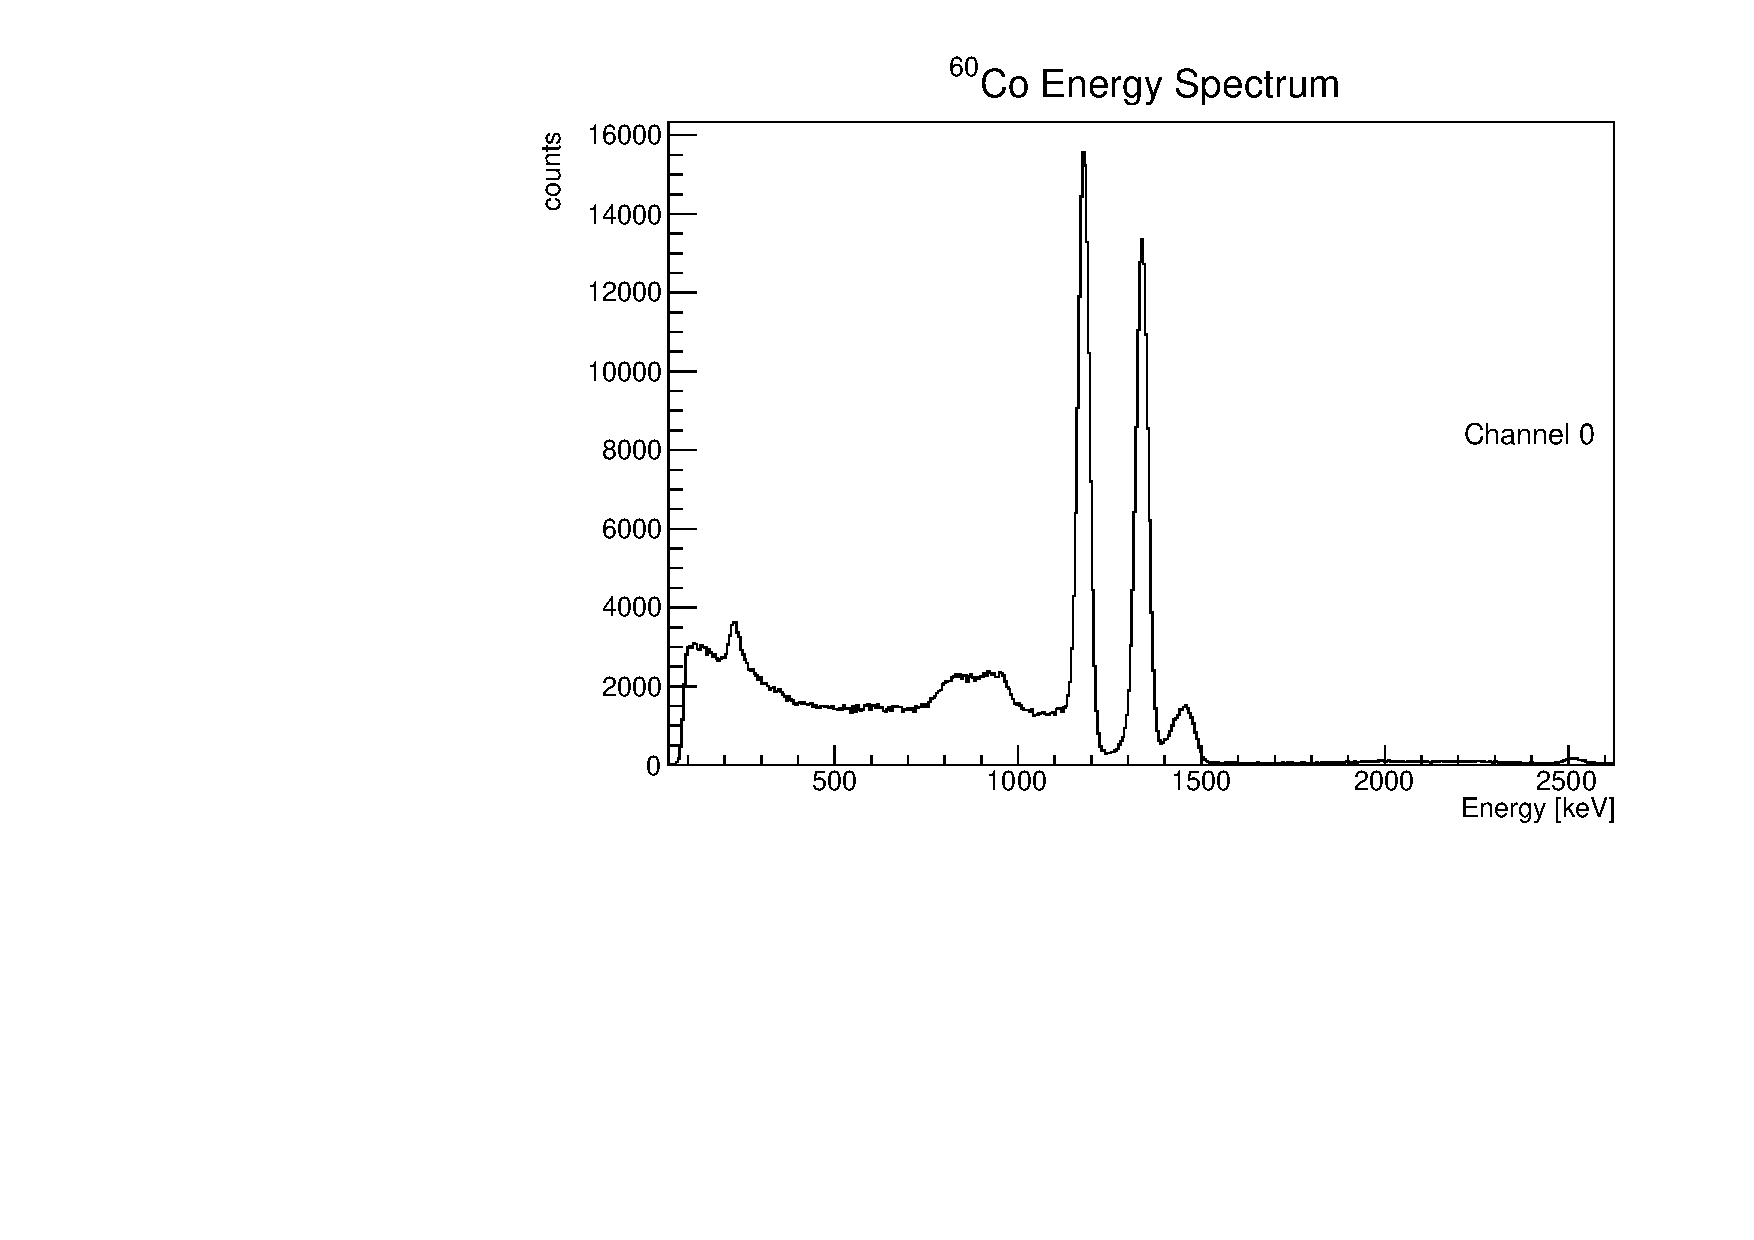
\includegraphics[scale=0.5]{Images/analysis/efficiency/Co.pdf}
    \caption{Energy spectrum of $^{60}$Co at 10 cm, for detector 0.}
    \label{fig:co}
\end{figure}

In order consider the summing up effect, the total efficiency is obtained using eq. \ref{eq:eta}

\begin{equation} \label{eq:eta}
    \eta=\eta_{peak} \, (1-\eta_{tot})
\end{equation}

where $\eta_{peak}$ is the efficiency obtained by considering the events in the peak and $\eta_{tot}$ is the efficiency obtained considering the total event of the spectrum as the number of event detected. \\

In this section, the data from $^{22}$Na source is also used. The results for all sources are shown in tab. \ref{tab:eff_nocoinc}. \\
The trend of the absolute efficiencies, shown in fig. \ref{fig:eff_nocoinc}, resembles the one obtained with the rough estimate in fig. \ref{fig:eff_rough}. We then estimate their compatibility for $^{60}$Co and $^{137}$Cs, and show the results in tab. \ref{tab:eff_comp}. The two methods provide compatible results.

\begin{figure}[H]
    \centering
    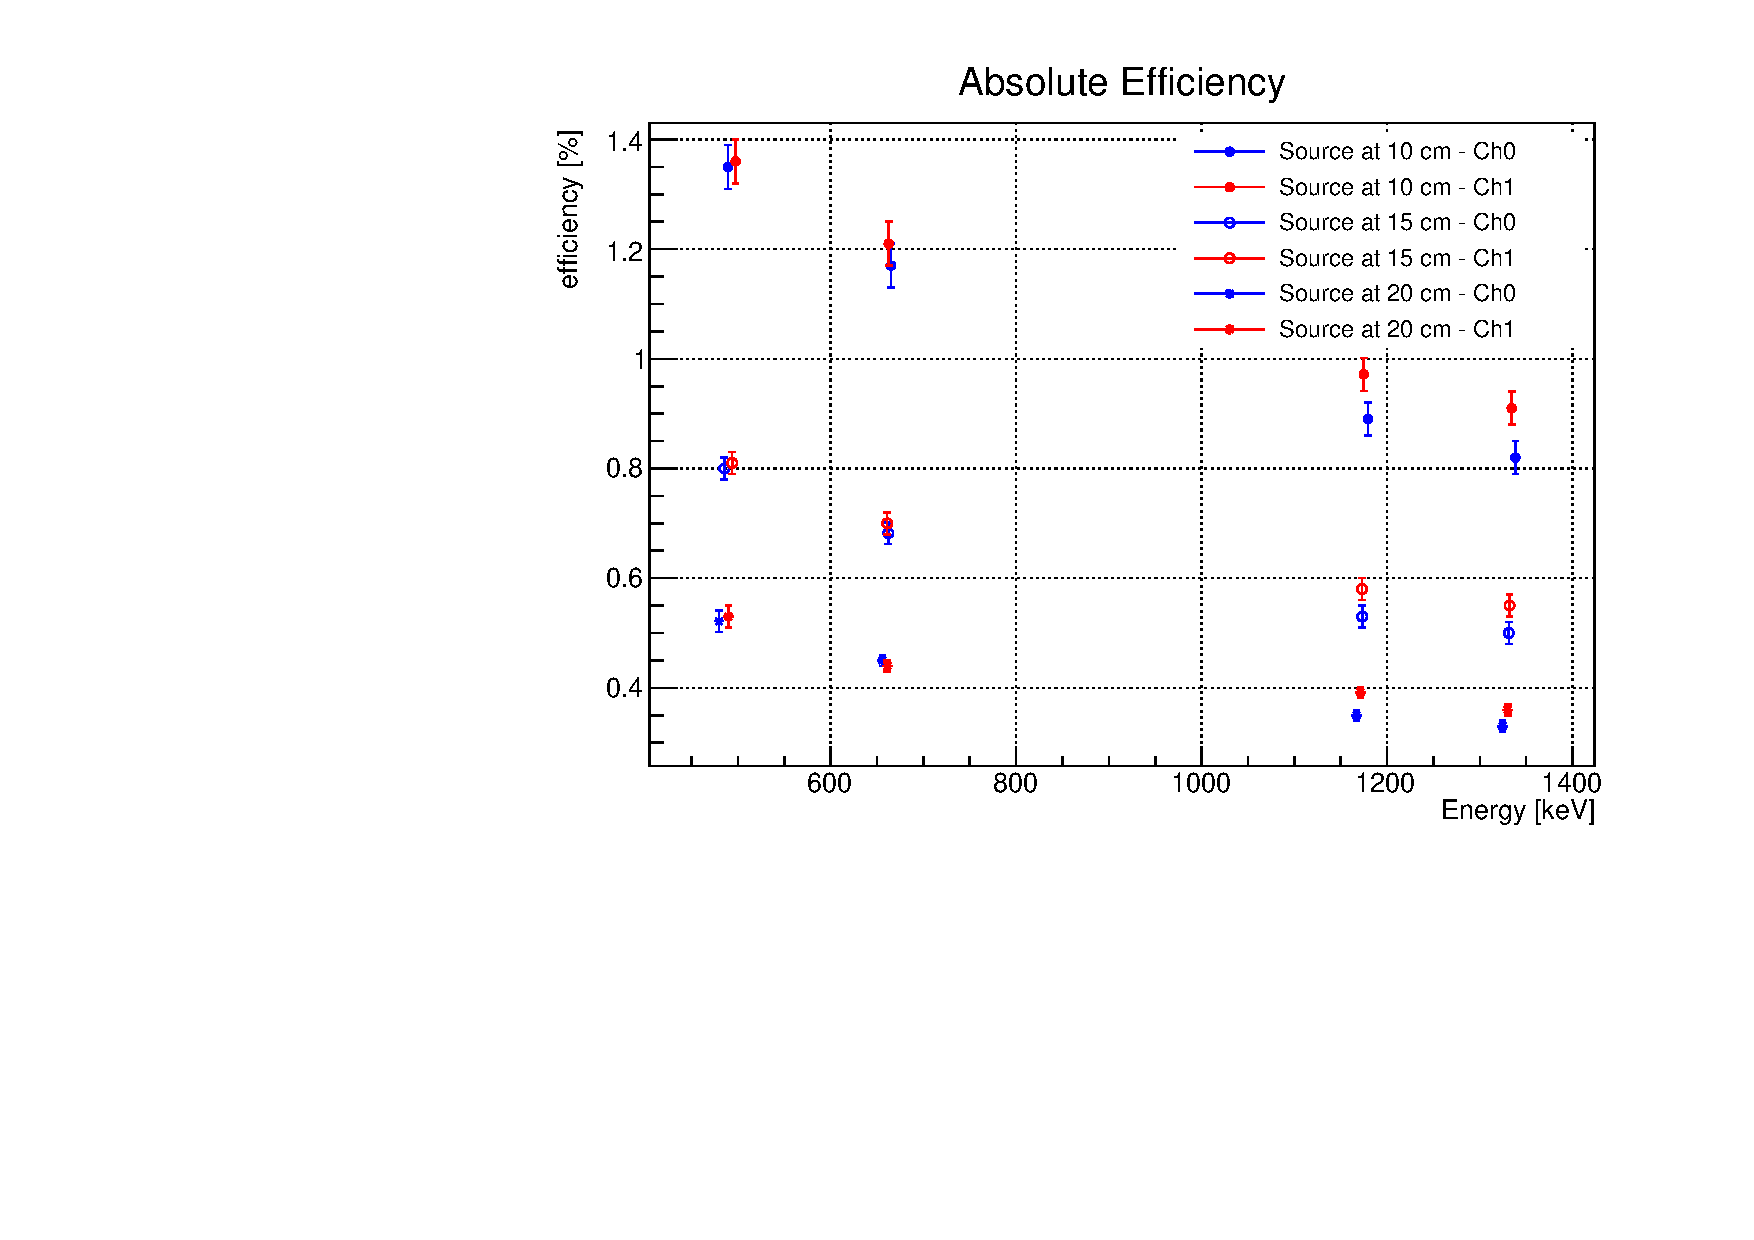
\includegraphics[scale=0.5]{Images/analysis/efficiency/Eff_nocoinc.pdf}
    \caption{Efficiency of the detectors, without using coincidences and considering summing up as in \ref{eq:eta}, with detector 0 in blue and detector 1 in red, for all the distances.}
    \label{fig:eff_nocoinc}
\end{figure}

\begin{figure}[H]
	\begin{minipage}[c]{0.35\linewidth}
    \centering
	\subfloat[][Sources at 10 cm.]{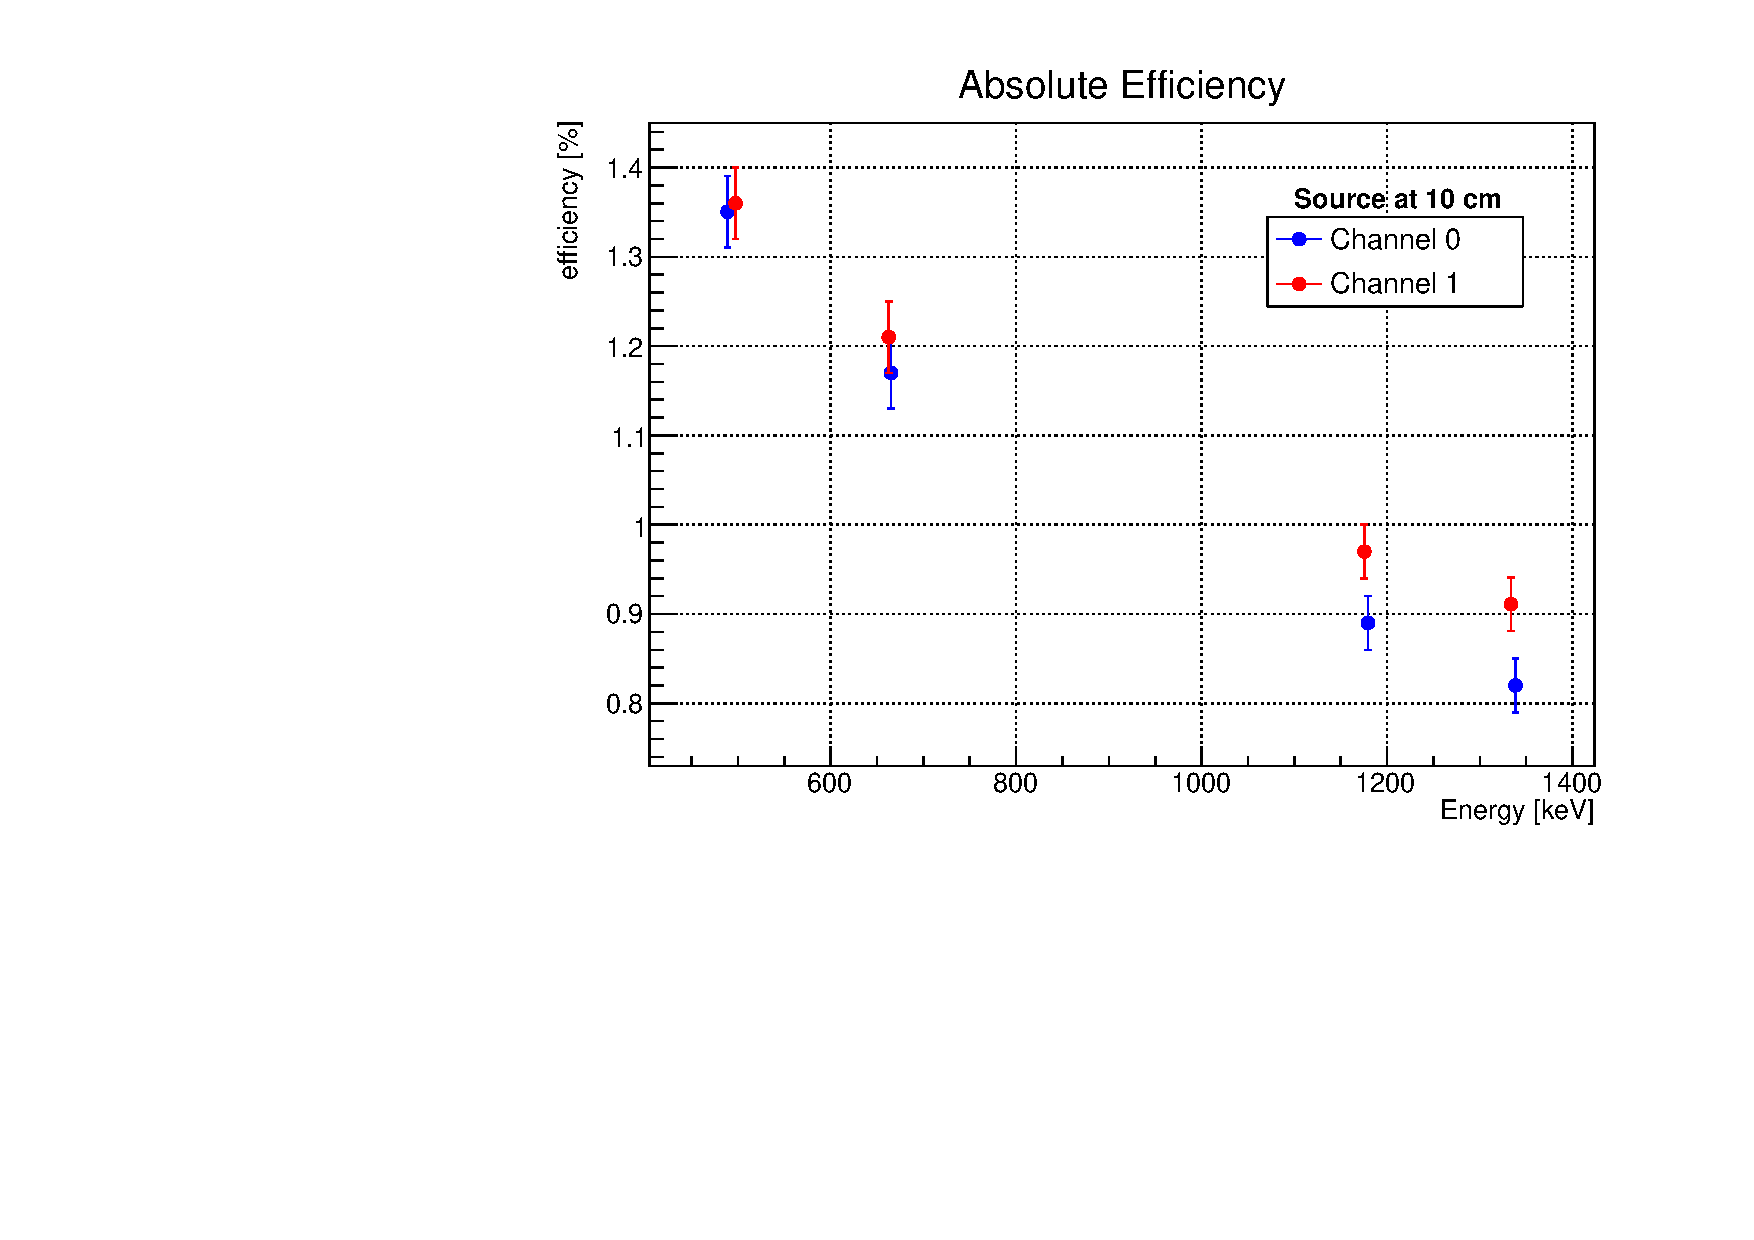
\includegraphics[width=0.95\textwidth]{Images/analysis/efficiency/eff_nocoinc_10.pdf} \label{fig:nocoinc_10} }
	\end{minipage}
	\begin{minipage}[]{0.35\linewidth}
	\centering
	\subfloat[][Sources at 15 cm.]{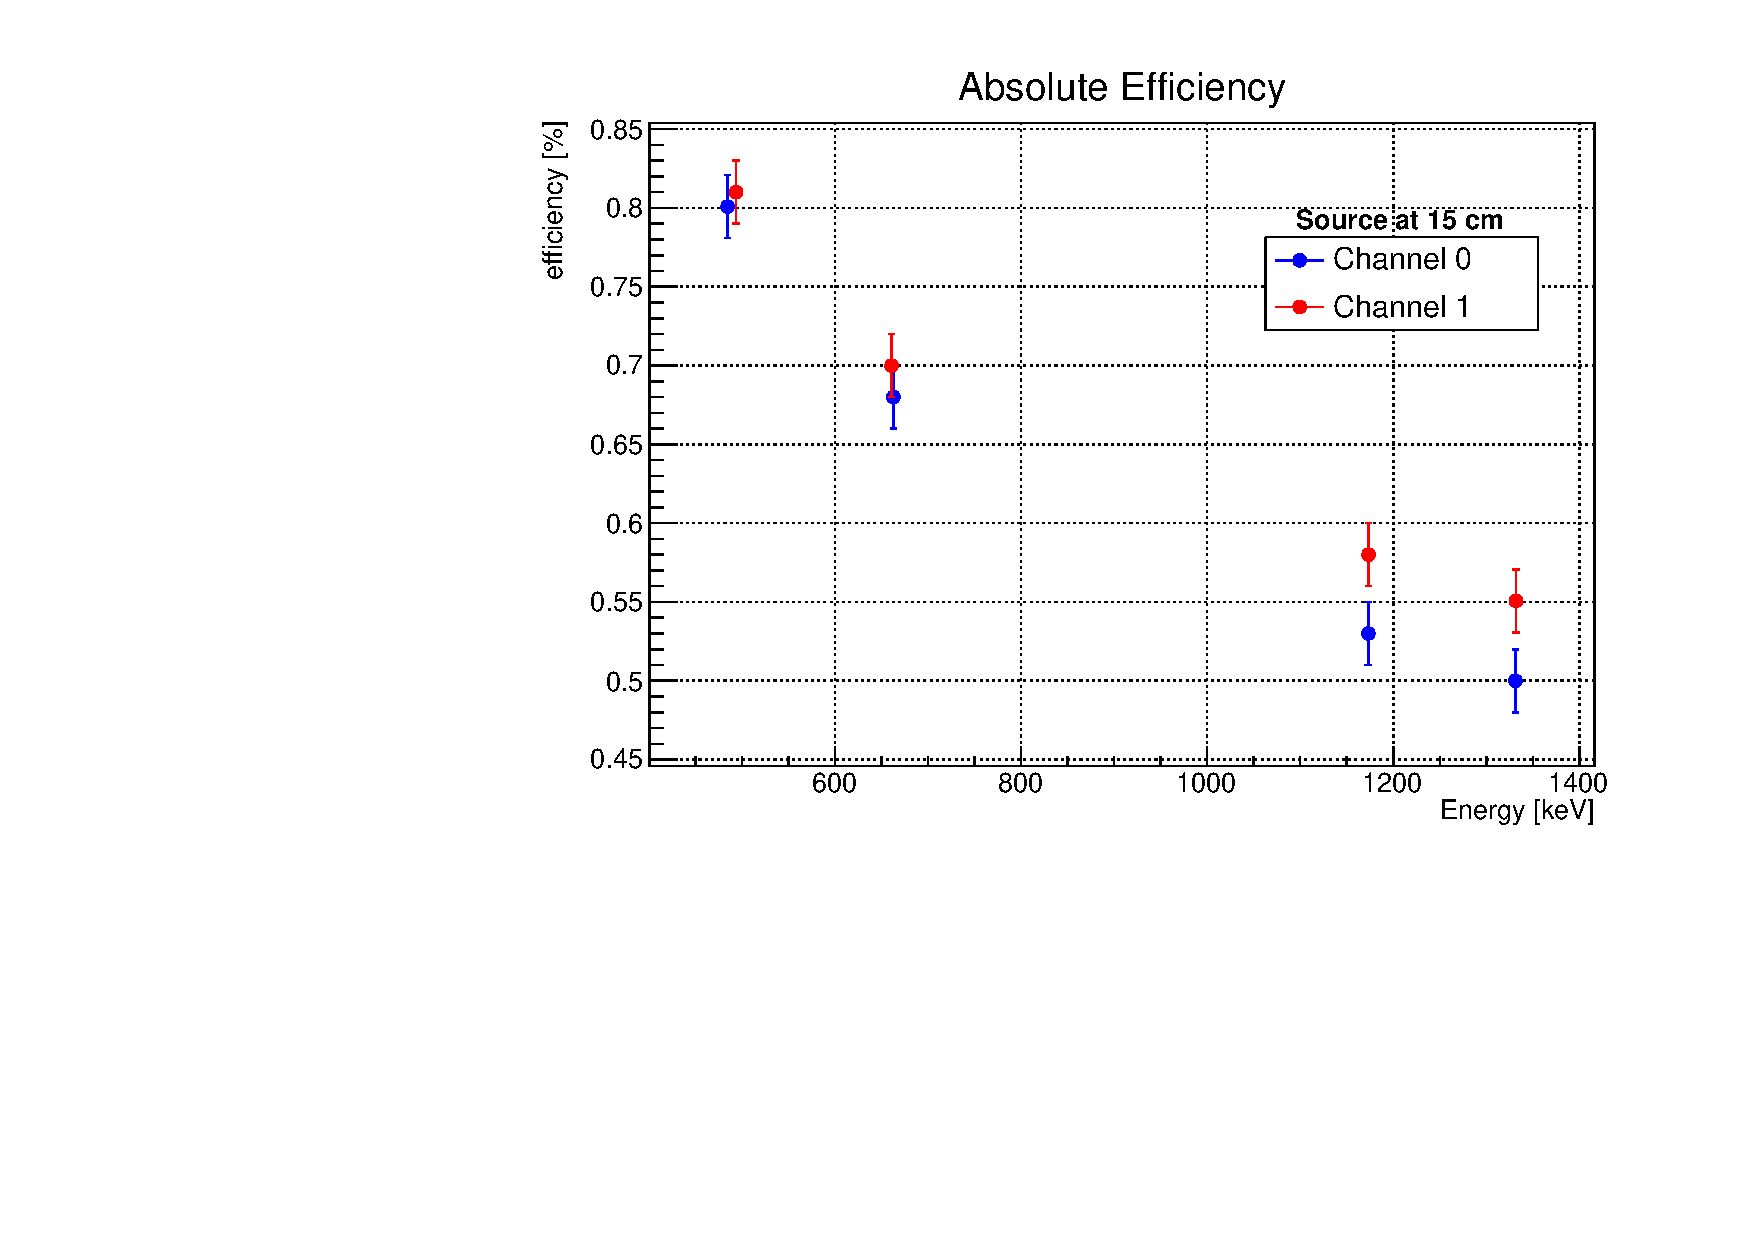
\includegraphics[width=0.95\textwidth]{Images/analysis/efficiency/eff_nocoinc_15.pdf}  \label{fig:nocoinc_15} }
	\end{minipage}
    \begin{minipage}[c]{0.35\linewidth}
    \centering
	\subfloat[][Source at 20 cm]{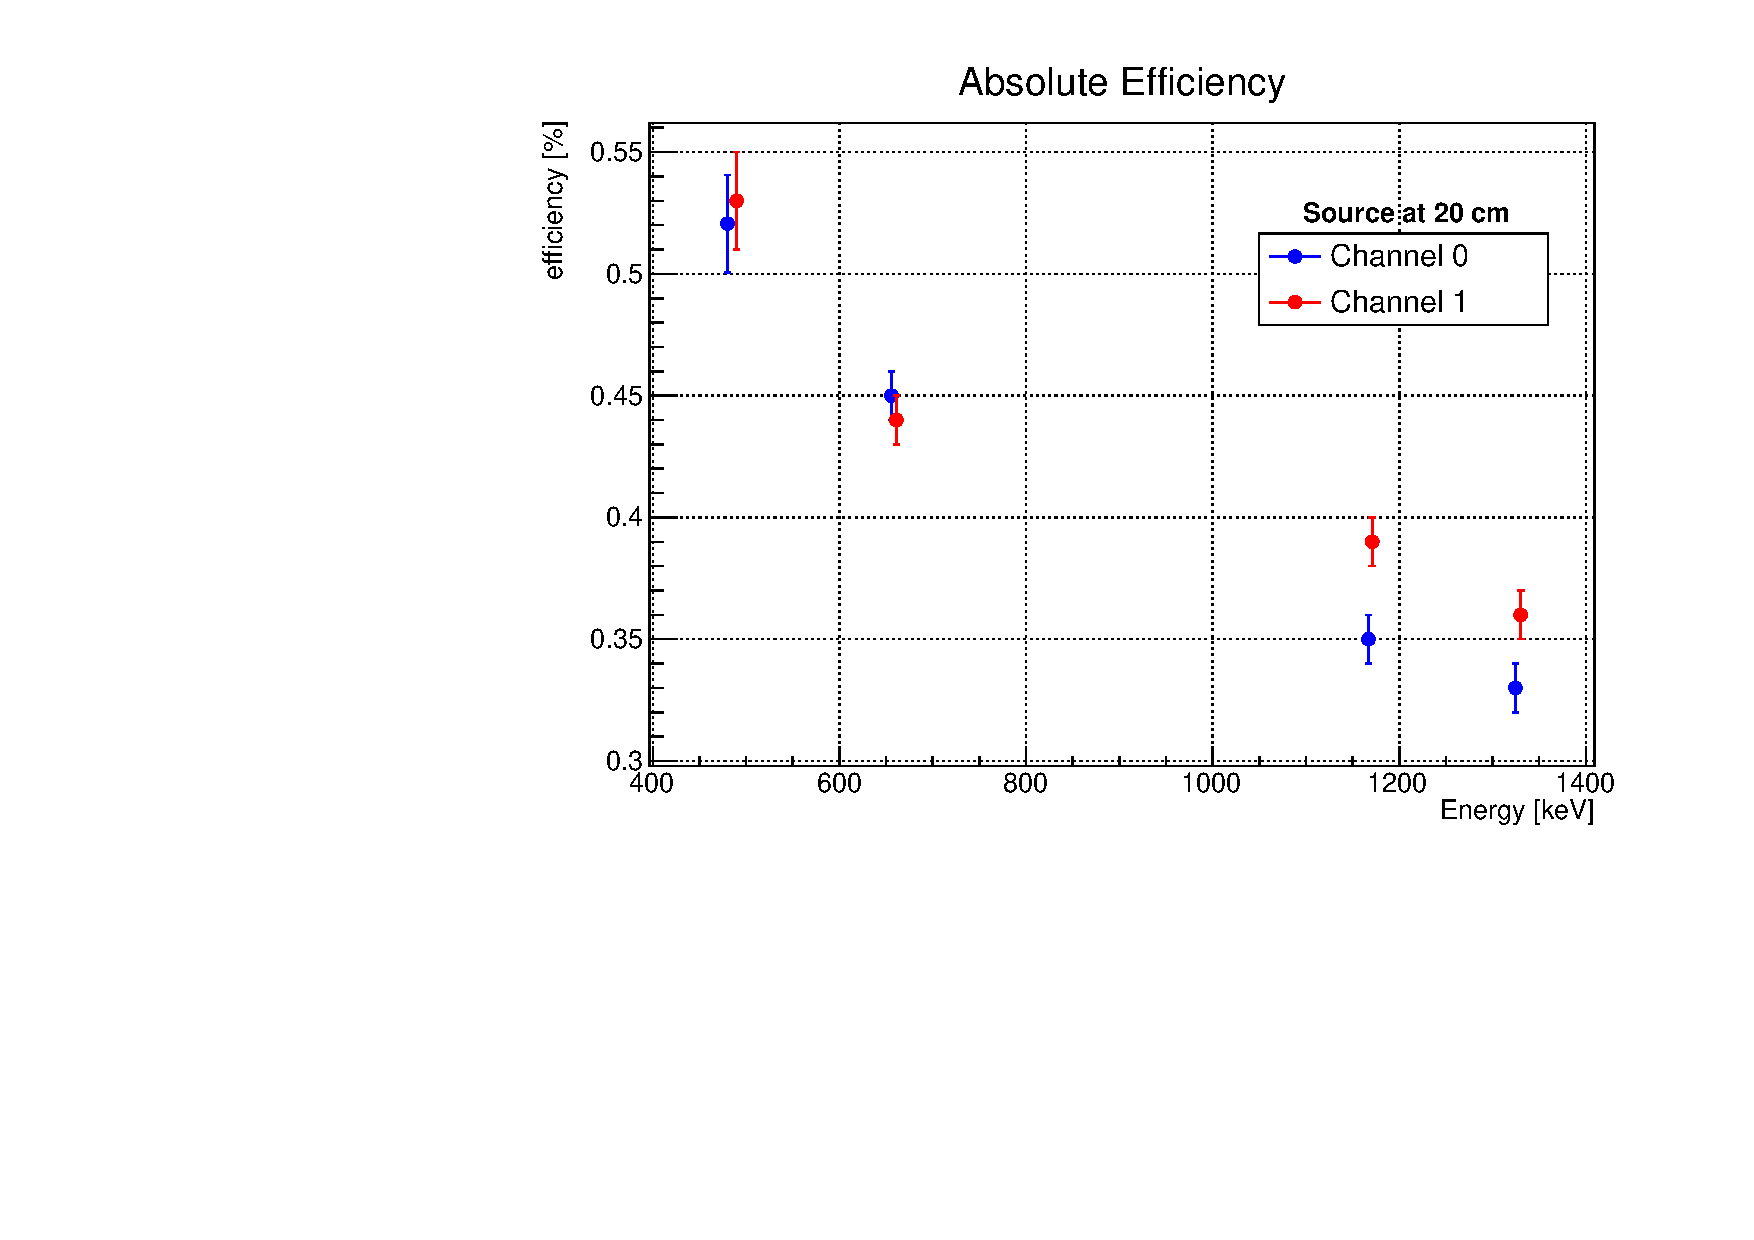
\includegraphics[width=0.95\textwidth]{Images/analysis/efficiency/eff_nocoinc_20.pdf}} \label{fig:nocoinc_20} 
	\end{minipage}
	\caption{Efficiency of the detectors, without using coincidences and considering summing up as in \ref{eq:eta}, with detector 0 in blue and detector 1 in red, at each different distances for each plot.}
    \label{fig:eff_nocoinc3}
	\end{figure}



\begin{table}[h]
    \begin{subtable}
        \centering
        \begin{tabular}{|c|c|c|c|}
        \hline
        & E [keV]  & eff [\%] &$\sigma_{eff}$ [\%]  \\
        \hline
        $^{22}$Na at 10 cm & 511 &1.35&0.04\\
        \hline
        $^{137}$Cs at 10 cm & 662 & 1.17 & 0.04\\
        \hline
        \multirow{2}{*}{$^{60}$Co at 10 cm}&1173 &0.89 & 0.03 \\ 
        &1332 &0.82 & 0.03 \\
        \hline
        $^{22}$Na at 15 cm & 511 &0.80&0.02\\
        \hline
        $^{137}$Cs at 15 cm & 662 & 0.68 & 0.02\\
        \hline
        \multirow{2}{*}{$^{60}$Co at 15 cm}&1173 &0.53 & 0.02 \\ 
        &1332 &0.50 & 0.02 \\
        \hline
        $^{22}$Na at 20 cm & 511 &0.52&0.02\\
        \hline
        $^{137}$Cs at 20 cm & 662 & 0.45 & 0.01\\
        \hline
        \multirow{2}{*}{$^{60}$Co at 20 cm}&1173 &0.35 & 0.01 \\
        &1332 &0.33 & 0.01 \\
        \hline
        \end{tabular}
    \end{subtable}
    \qquad
    \qquad
    \qquad
    \begin{subtable}
        \centering
        \begin{tabular}{|c|c|c|c|}
        \hline
        & E [keV]  & eff [\%] &$\sigma_{eff}$ [\%]  \\
        \hline
        $^{22}$Na at 10 cm & 511 &1.36&0.04\\
        \hline
        $^{137}$Cs at 10 cm & 662 & 1.21 & 0.04\\
        \hline
        \multirow{2}{*}{$^{60}$Co at 10 cm}&1173 &0.97 & 0.03 \\ 
        &1332 &0.91 & 0.03 \\
        \hline
        $^{22}$Na at 15 cm & 511 &0.81&0.02\\
        \hline
        $^{137}$Cs at 15 cm & 662 &0.70 & 0.02\\
        \hline
        \multirow{2}{*}{$^{60}$Co at 15 cm}&1173 &0.58 & 0.02 \\ 
        &1332 &0.55 & 0.02 \\
        \hline
        $^{22}$Na at 20 cm & 511 &0.53&0.02\\
        \hline
        $^{137}$Cs at 20 cm & 662 & 0.44 & 0.01\\
        \hline
        \multirow{2}{*}{$^{60}$Co at 20 cm}&1173 &0.39 & 0.01 \\
        &1332 &0.36 & 0.01 \\
        \hline
        \end{tabular}
     \end{subtable}
     \caption{Values of efficiency for all the sources at different distances, considering summing up, for detector 0 and 1 respectively.}
     \label{tab:eff_nocoinc}
\end{table}

\begin{table}[h]
    \begin{subtable}
        \centering
        \begin{tabular}{|c|c|c|c|}
        \hline
        $\lambda$& 10 cm & 15 cm & 20 cm  \\
        \hline
        662 keV & 0.7 & 0.5 & 0.4 \\
        1173 keV& 1.7 & 1.1 & 0.8 \\
        1132 keV& 1.8 & 1.1 & 0.8 \\
        \hline
        \end{tabular}
    \end{subtable}
    \qquad
    \qquad
    \qquad
    \begin{subtable}
        \centering
        \begin{tabular}{|c|c|c|c|}
        \hline
        $\lambda$ & 10 cm & 15 cm & 20 cm \\
        \hline
        662 keV & 0.8 & 0.5 & 0.4 \\
        1173 keV& 1.8 & 1.2 & 0.8 \\
        1132 keV& 1.9 & 1.2 & 0.8 \\
        \hline
        \end{tabular}
     \end{subtable}
     \caption{Compatibility between the efficiencies obtained in sec. \ref{sub:rough} and sec. \ref{sub:nocoinc}, between every value at each distance and energy, with detector 0 in the first table and detector 1 in the second.}
     \label{tab:eff_comp}
\end{table}



\subsection{With Coincidences}

In this section we want to compute the efficiency of the detectors more accurately by exploiting the coincidences between the gamma emissions in the decays of $^{22}$Na and $^{60}$Co. In sec. \ref{sec:timing} we established that two events from different channels can be considered in coincidence if their time difference is less than 16 ns. Since we want to analyze only the events in coincidence, we plot the energy spectra for each channel, imposing the condition that an event in the other channel must have a time difference smaller then 16 ns (fig.\ref{fig:coinc_spectra}). 

\begin{figure}[H]
	\begin{minipage}[c]{0.5\linewidth}
	\subfloat[][$^{60}$Co source at 10 cm.]{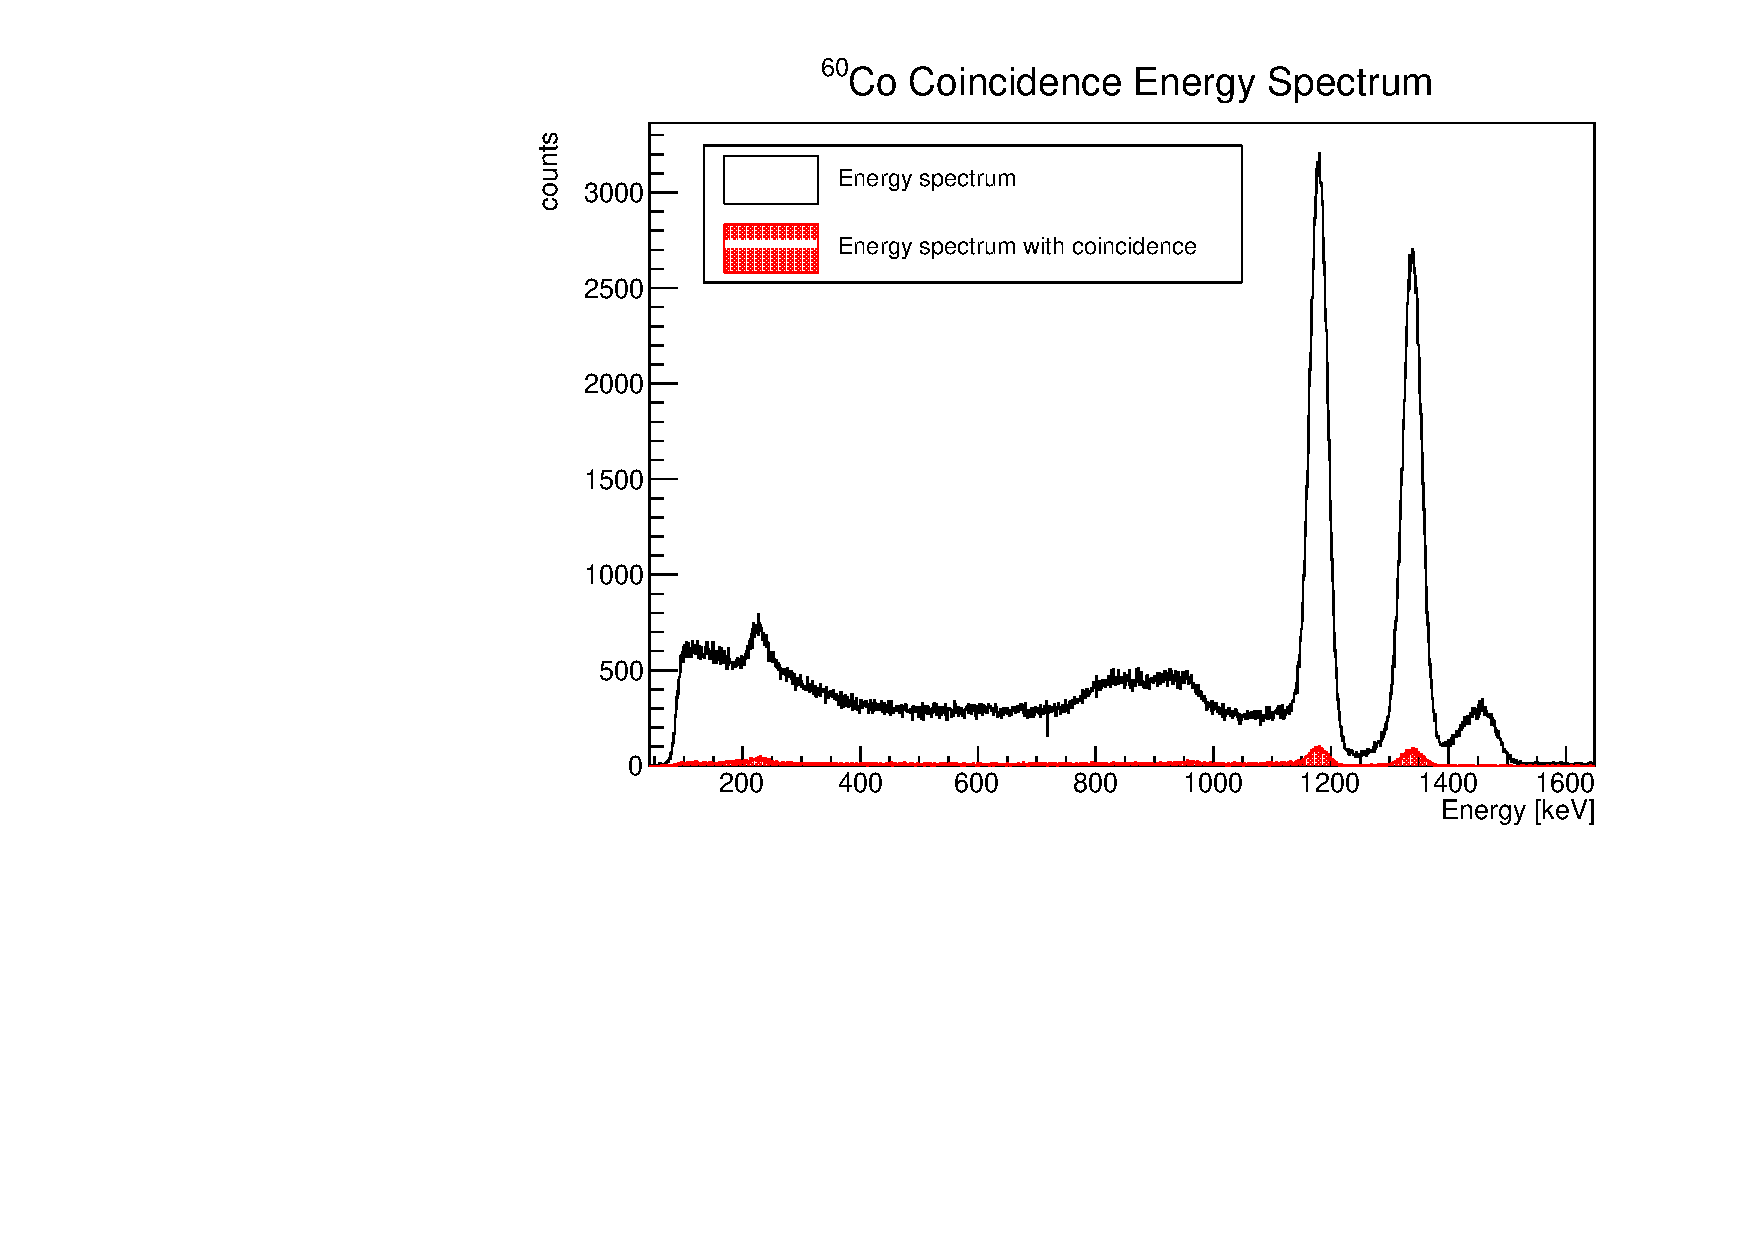
\includegraphics[width=0.9\textwidth]{Images/analysis/efficiency/Co_coinc_both.pdf} \label{fig:Co_coinc} }
	\end{minipage}
	\begin{minipage}[]{0.5\linewidth}
	\centering
	\subfloat[][$^{22}$Na source at 10 cm.]{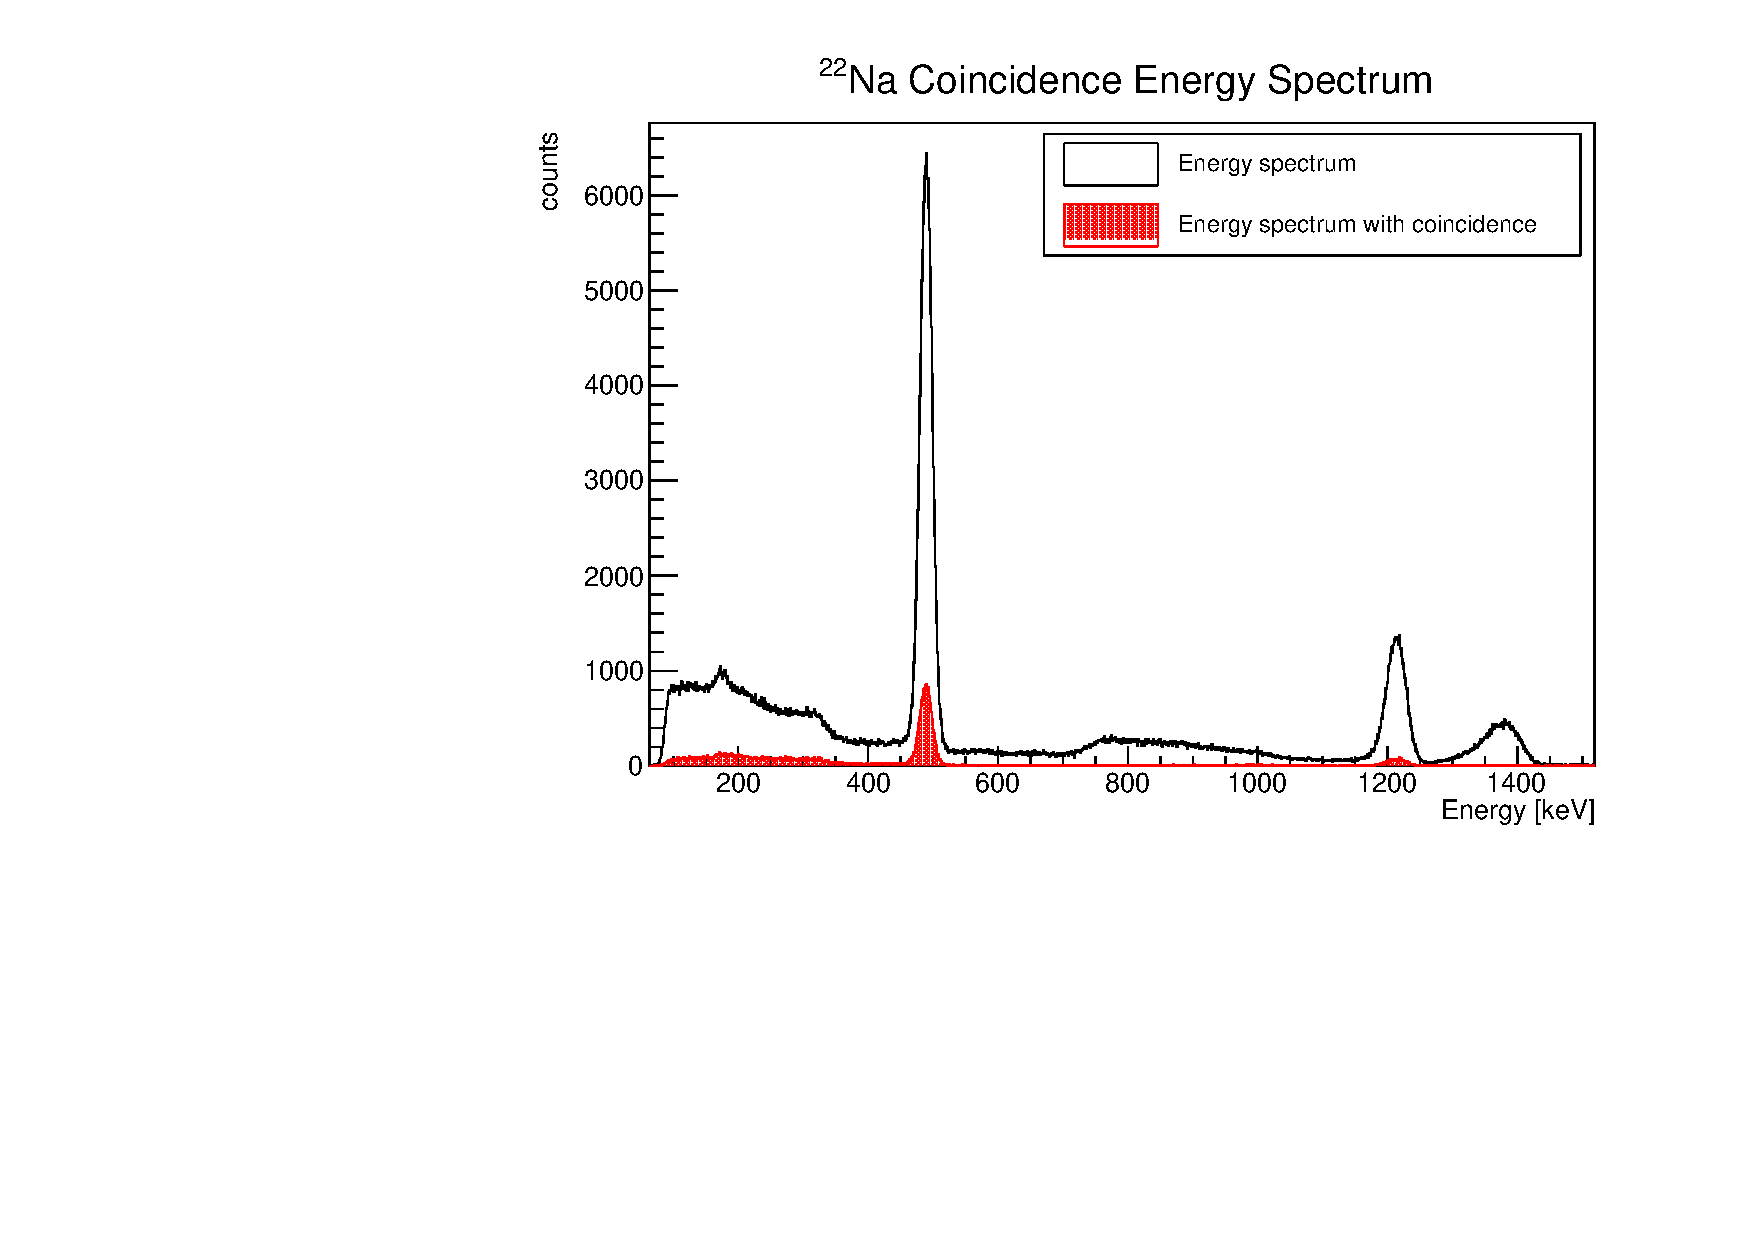
\includegraphics[width=0.9\textwidth]{Images/analysis/efficiency/Na_coinc_both.pdf}  \label{fig:Na_coinc} }
	\end{minipage}
	\caption{Comparison between the initial energy spectra of $^{60}$Co and $^{22}$Na, in black, and the energy spectra obtained imposing coincidence between the two detectors, in red, both spectra regard detector 0.}
    \label{fig:coinc_spectra}
	\end{figure}

Once we obtain these spectra, we estimate the number of events corresponding to each energy, evaluating the areas of the peak and taking into account the summing up as in eq. \ref{eq:eta}. We can thus estimate the efficiencies (tab.\ref{table:eff_coin}), and plot their trend (fig. \ref{fig:eff_coinc}). \\

We can observe that the values of the efficiencies are smaller than the ones obtained in \ref{sub:rough} and \ref{sub:nocoinc}. This is due to the fact that when we impose the condition on coincidence the number of events considered gets significantly smaller than the one used before, as we are taking away irrelevant events. \\
We can also observe that the decrease in efficiency is more substantial for the efficiencies corresponding to the energies of $^{60}$Co. This is due to the fact that we are not taking into account the geometric distribution of the photons. In the $^{22}$Na decay the gammas are emitted in opposite direction, so that when one photon arrives to one detector, so does the other photon in the second detector, meaning that by imposing coincidence we cut mainly background events. In the case of $^{60}$Co, conversely, the gammas are emitted with an angular distribution, so that when one arrives to one detector it is not certain that the other will hit to the other detector. This means that also these event of non-opposite photons are cut away from the analysis, resulting in a smaller number of events in the peaks and therefore in a smaller efficiency.

\begin{figure}[H]
    \centering
    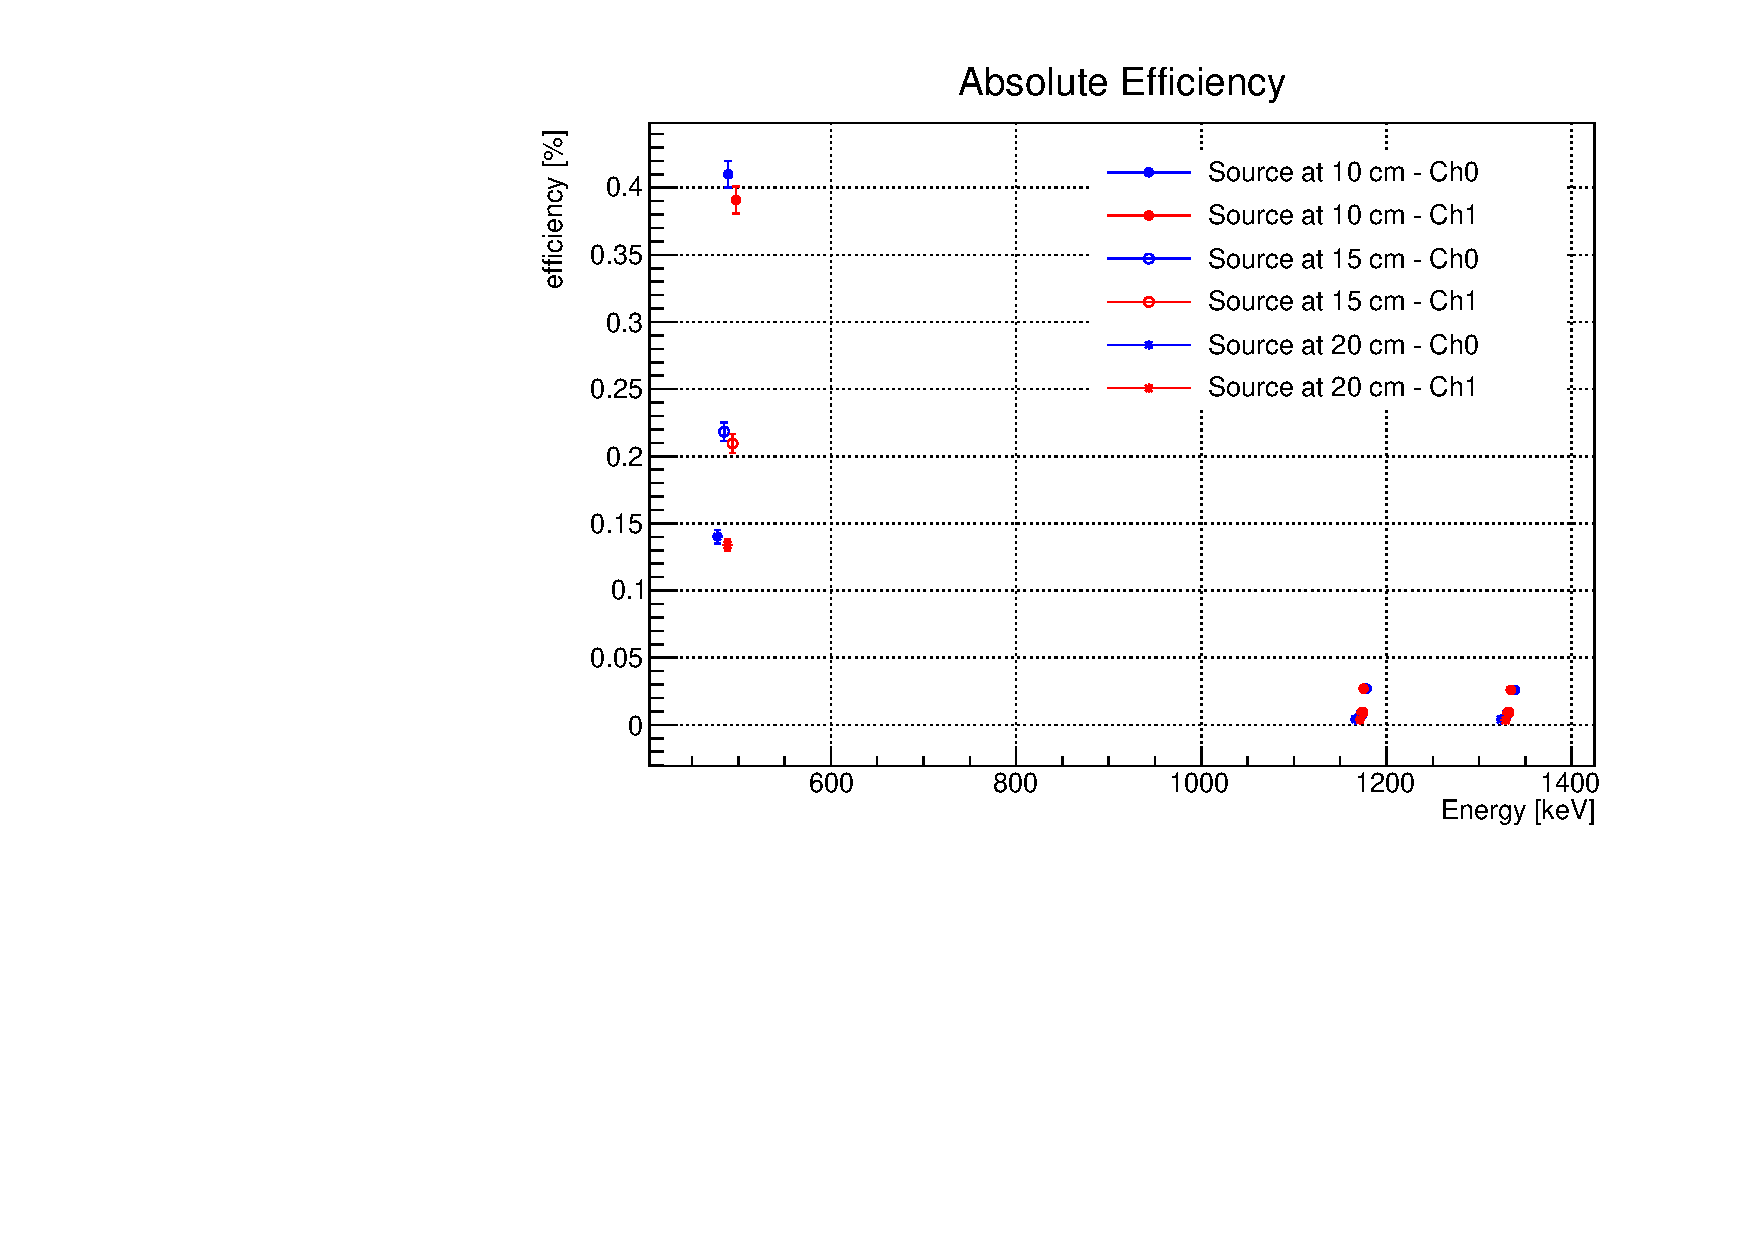
\includegraphics[scale=0.5]{Images/analysis/efficiency/Eff_coinc.pdf}
    \caption{Efficiency of the detectors, imposing coincidences and considering summing up as in \ref{eq:eta}, with detector 0 in blue and detector 1 in red, for all the distances.}
    \label{fig:eff_coinc}
\end{figure}

\begin{figure}[H]
	\begin{minipage}[c]{0.35\linewidth}
    \centering
	\subfloat[][Sources at 10 cm.]{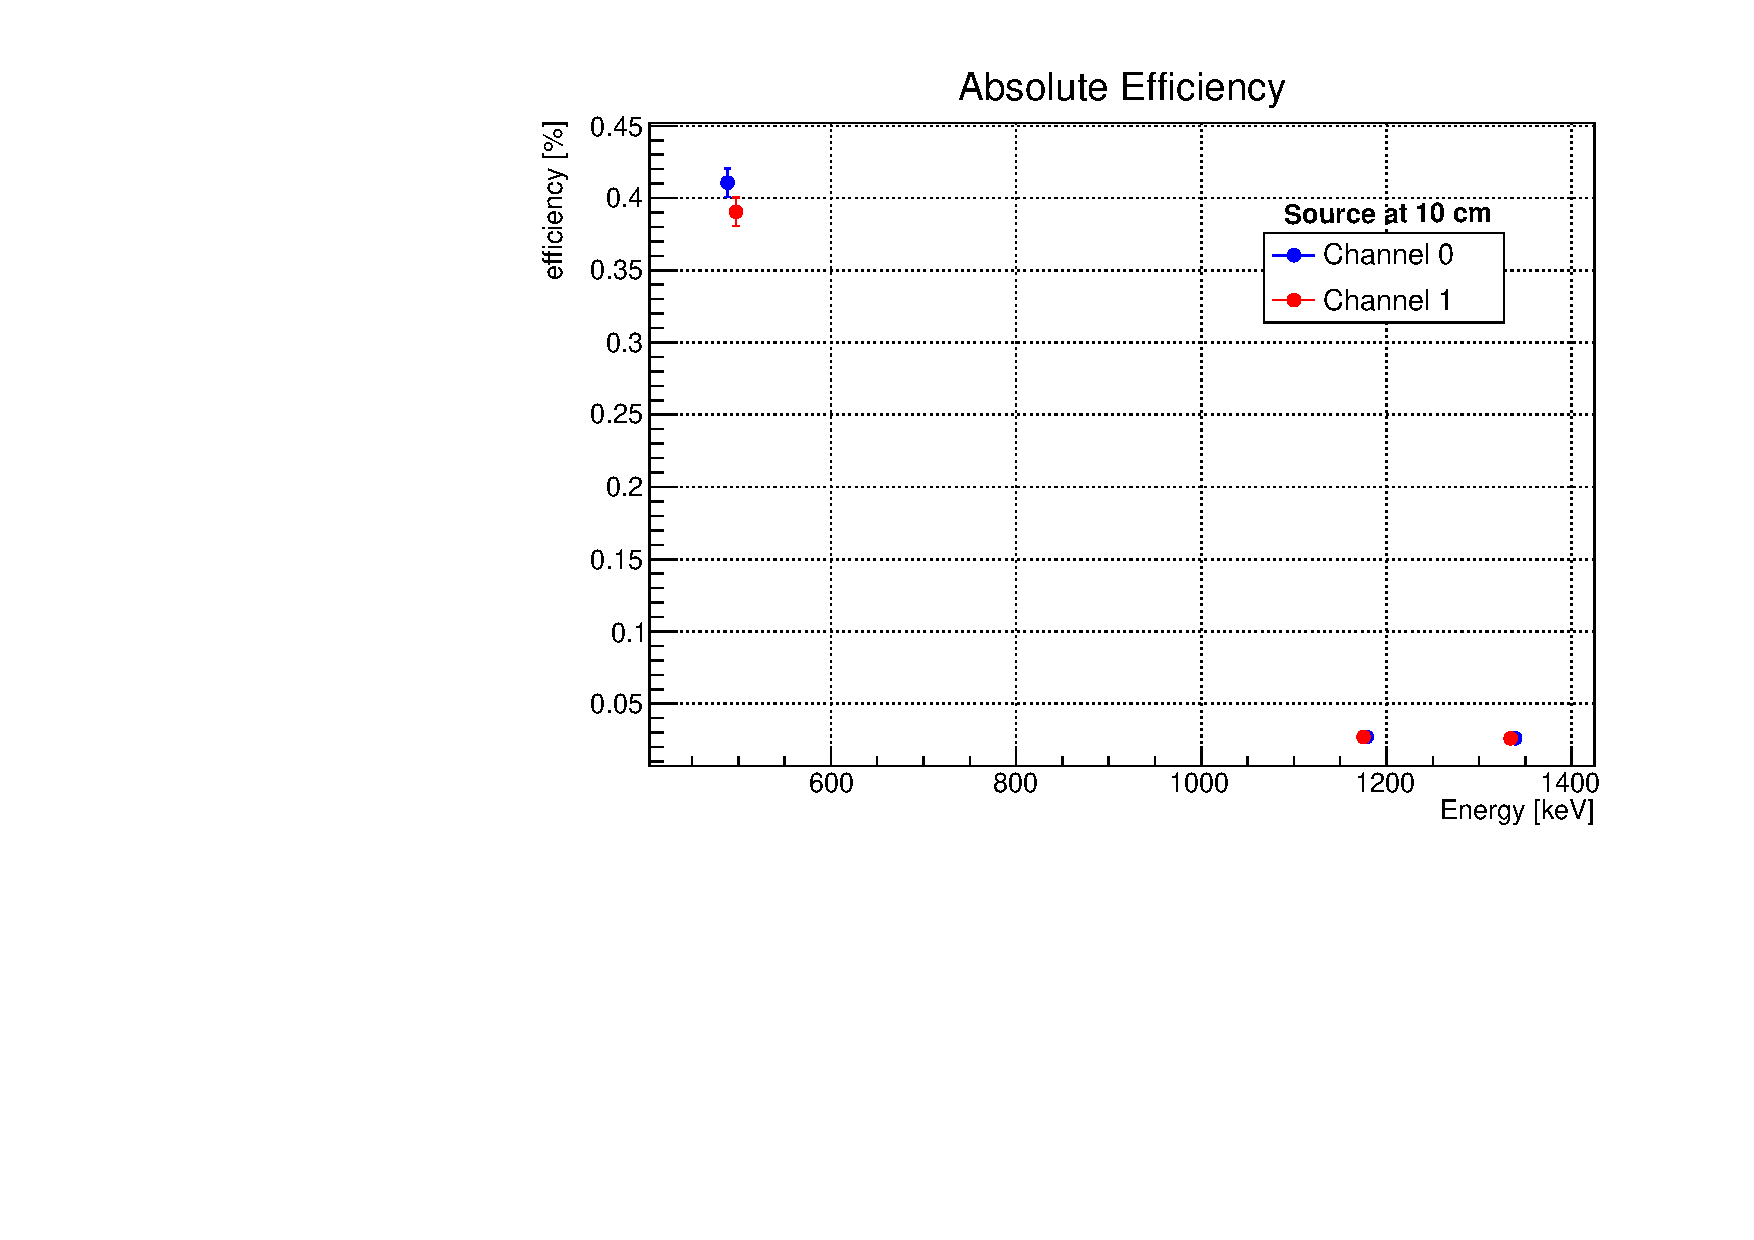
\includegraphics[width=0.95\textwidth]{Images/analysis/efficiency/eff_coinc_10.pdf} \label{fig:coinc_10} }
	\end{minipage}
	\begin{minipage}[]{0.35\linewidth}
	\centering
	\subfloat[][Sources at 15 cm.]{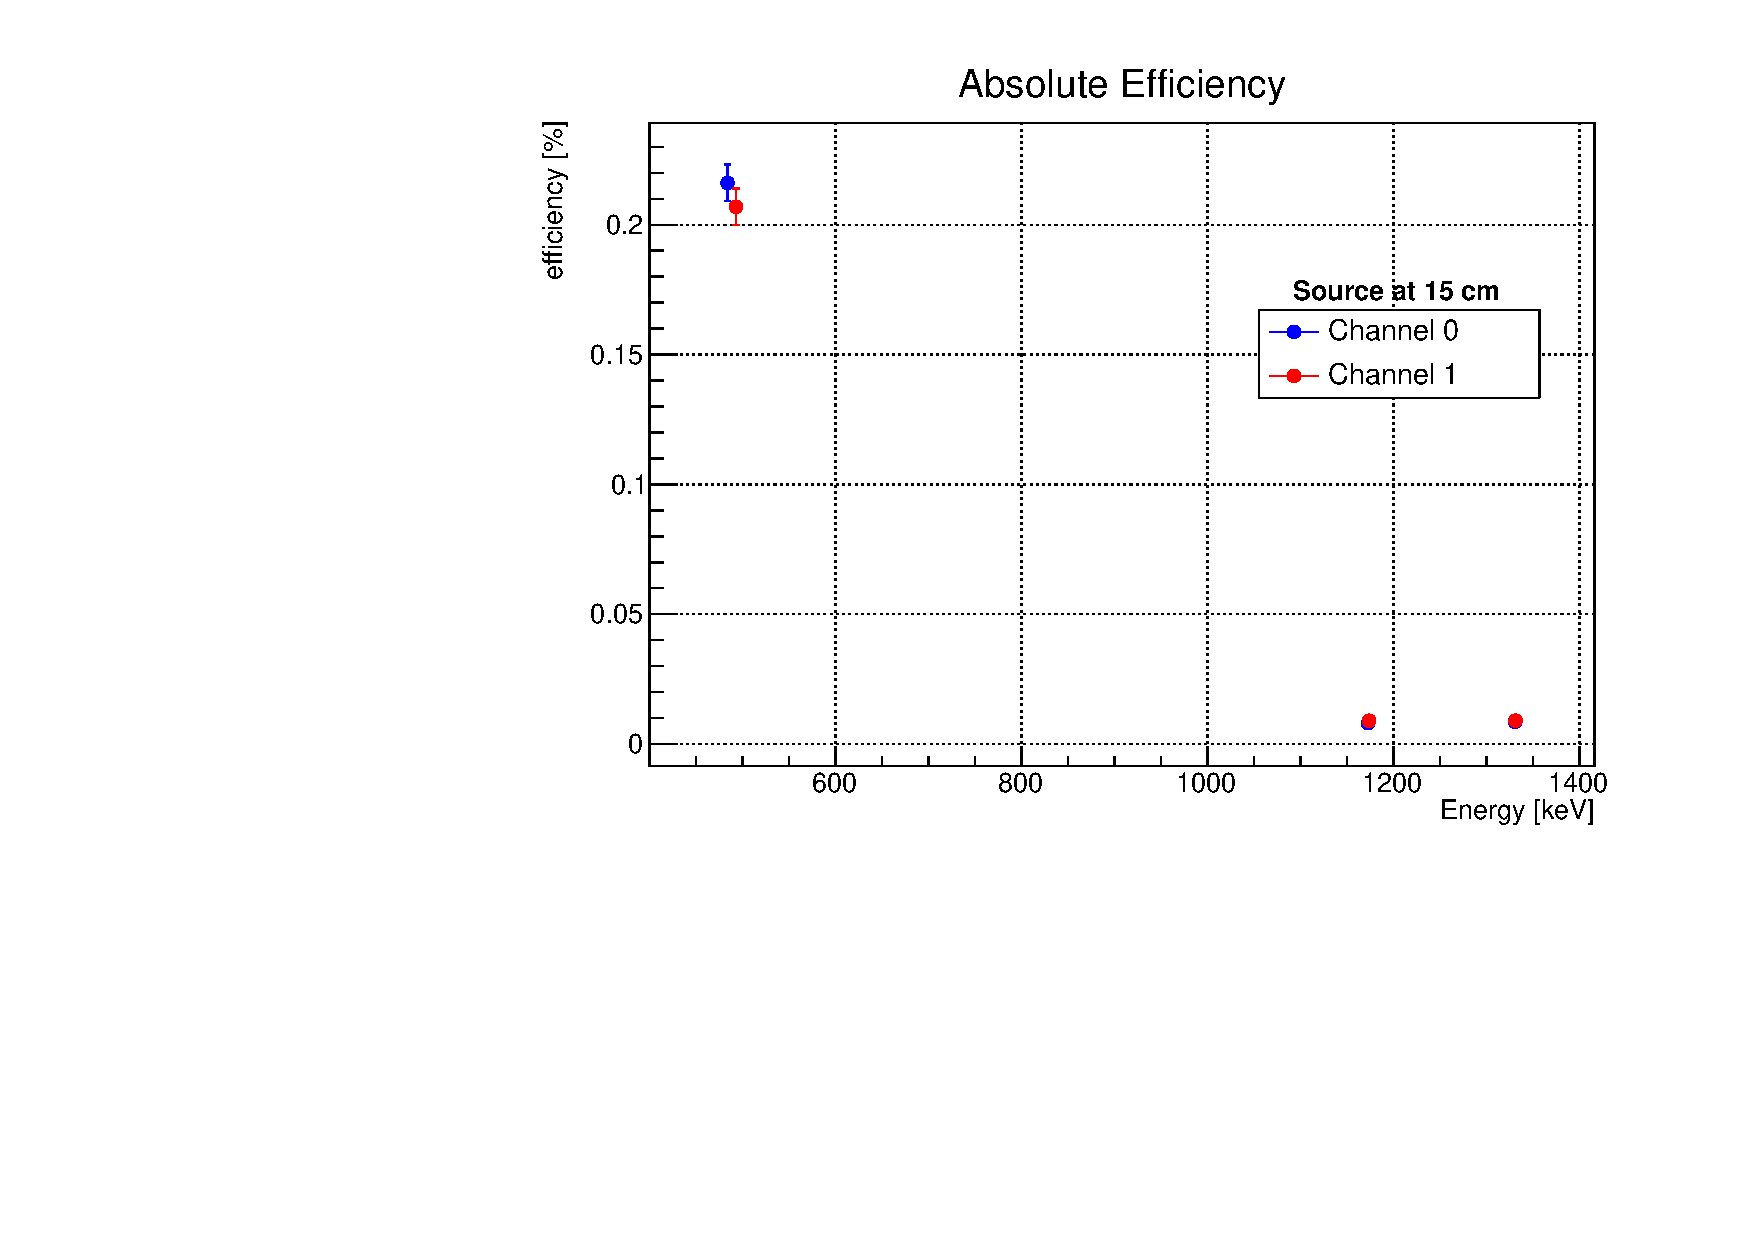
\includegraphics[width=0.95\textwidth]{Images/analysis/efficiency/eff_coinc_15.pdf}  \label{fig:coinc_15} }
	\end{minipage}
    \begin{minipage}[c]{0.35\linewidth}
    \centering
	\subfloat[][Source at 20 cm]{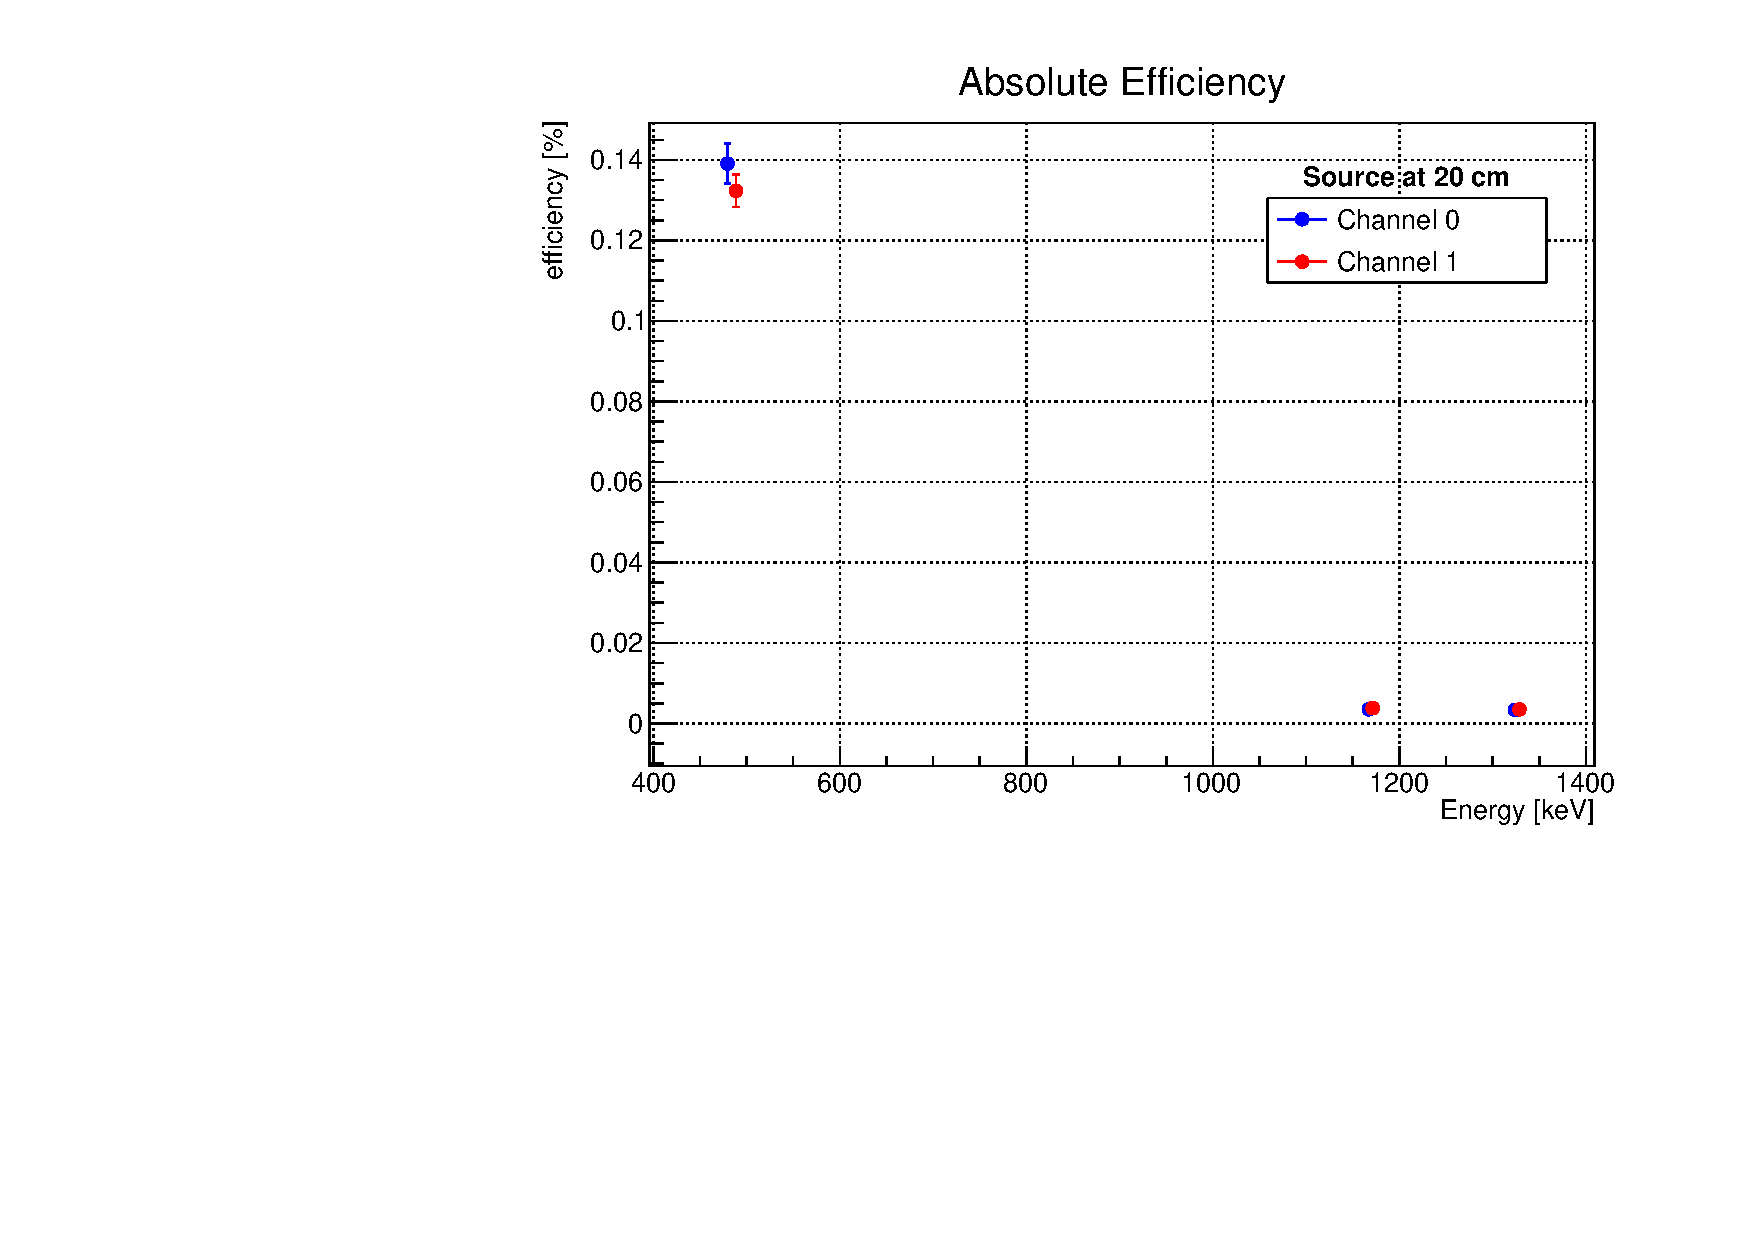
\includegraphics[width=0.95\textwidth]{Images/analysis/efficiency/eff_coinc_20.pdf}} \label{fig:coinc_20} 
	\end{minipage}
	\caption{Efficiency of the detectors, imposing coincidences and considering summing up as in \ref{eq:eta}, with detector 0 in blue and detector 1 in red, at each different distances for each plot.}
    \label{fig:eff_coinc3}
	\end{figure}


\begin{table}[h]
    \begin{subtable}
        \centering
        \begin{tabular}{|c|c|c|c|}
        \hline
        & E [keV]  & eff [\%] &$\sigma_{eff}$ [\%]  \\
        \hline
        $^{22}$Na at 10 cm & 511 &0.41&0.01\\
        \hline
        \multirow{2}{*}{$^{60}$Co at 10 cm}&1173 &0.027 & 0.001 \\ 
        &1332 &0.026 & 0.001 \\
        \hline
        $^{22}$Na at 15 cm & 511 &0.216&0.007\\
        \hline
        \multirow{2}{*}{$^{60}$Co at 15 cm}&1173 &0.008 & 0.001 \\ 
        &1332 &0.0086 & 0.0005 \\
        \hline
        $^{22}$Na at 20 cm & 511 &0.139&0.005\\
        \hline
        \multirow{2}{*}{$^{60}$Co at 20 cm}&1173 &20.0035 & 0.0003 \\
        &1332 &20.0034 & 0.0003 \\
        \hline
        \end{tabular}
    \end{subtable}
    \qquad
    \qquad
    \qquad
    \begin{subtable}
        \centering
        \begin{tabular}{|c|c|c|c|}
        \hline
        & E [keV]  & eff [\%] &$\sigma_{eff}$ [\%]  \\
        \hline
        $^{22}$Na at 10 cm & 511 &0.39&0.01\\
        \hline
        \multirow{2}{*}{$^{60}$Co at 10 cm}&1173 &0.027 & 0.001 \\ 
        &1332 &0.026 & 0.001 \\
        \hline
        $^{22}$Na at 15 cm & 511 &0.207&0.007\\
        \hline
        \multirow{2}{*}{$^{60}$Co at 15 cm}&1173 &0.009 & 0.001 \\ 
        &1332 &0.009 & 0.001 \\
        \hline
        $^{22}$Na at 20 cm & 511 &0.132&0.004\\
        \hline
        \multirow{2}{*}{$^{60}$Co at 20 cm}&1173 &0.0038 & 0.0003 \\
        &1332 &0.0035 & 0.0003 \\
        \hline
        \end{tabular}
     \end{subtable}
     \caption{Values of efficiency for the $^{60}$Co and $^{22}$Na source at different distances, imposing the coincidence between the detectors, for detector 0 and 1, respectively.}
     \label{table:eff_coin}
\end{table}


\subsection{With Coincidences and Condition on Energy}

To have a more refined efficiency we can impose a condition on the energy. In particular, we want to see the energy spectrum of a detector (b) when the other (a) sees a particular gamma. In this way the number of emitted events used to calculate the efficiency is not the number of events produced by the source, but is the number of events in an energy range detected by detector a. To do this calculation we plot the energy spectrum of detector b (fig. \ref{fig:coinc_spectra_all}-\ref{fig:coinc_spectra_all_log}), when we have temporal coincidences and when the other detector (a) registers events within $2\sigma$ from the value of the peak of interest. We then calculate the area of the peak of the spectrum for detector b with the condition required, as the number of detected events and we divide it by the number of events in the energy range of the spectrum of detector a, obtaining the efficiencies shown in tab. \ref{tab:eff_coin_en} and in fig. \ref{fig:eff_all}. \\

We can see that the values of efficiencies for $^{22}$Na, despite the source being moved further away, remain roughly the same. This is due to the fact that we are taking the ratio of events between the two detectors, so even though the solid angle subtended by the single detectors gets smaller, the two geometric factors cancel each other out and the efficiency remains constant.
This is not true for $^{60}$Co, as the photons are not necessarily emitted in opposite directions so the decreasing solid angle plays a role.  

\begin{figure}[H]
	\begin{minipage}[c]{0.5\linewidth}
	\subfloat[][$^{60}$Co source at 10 cm.]{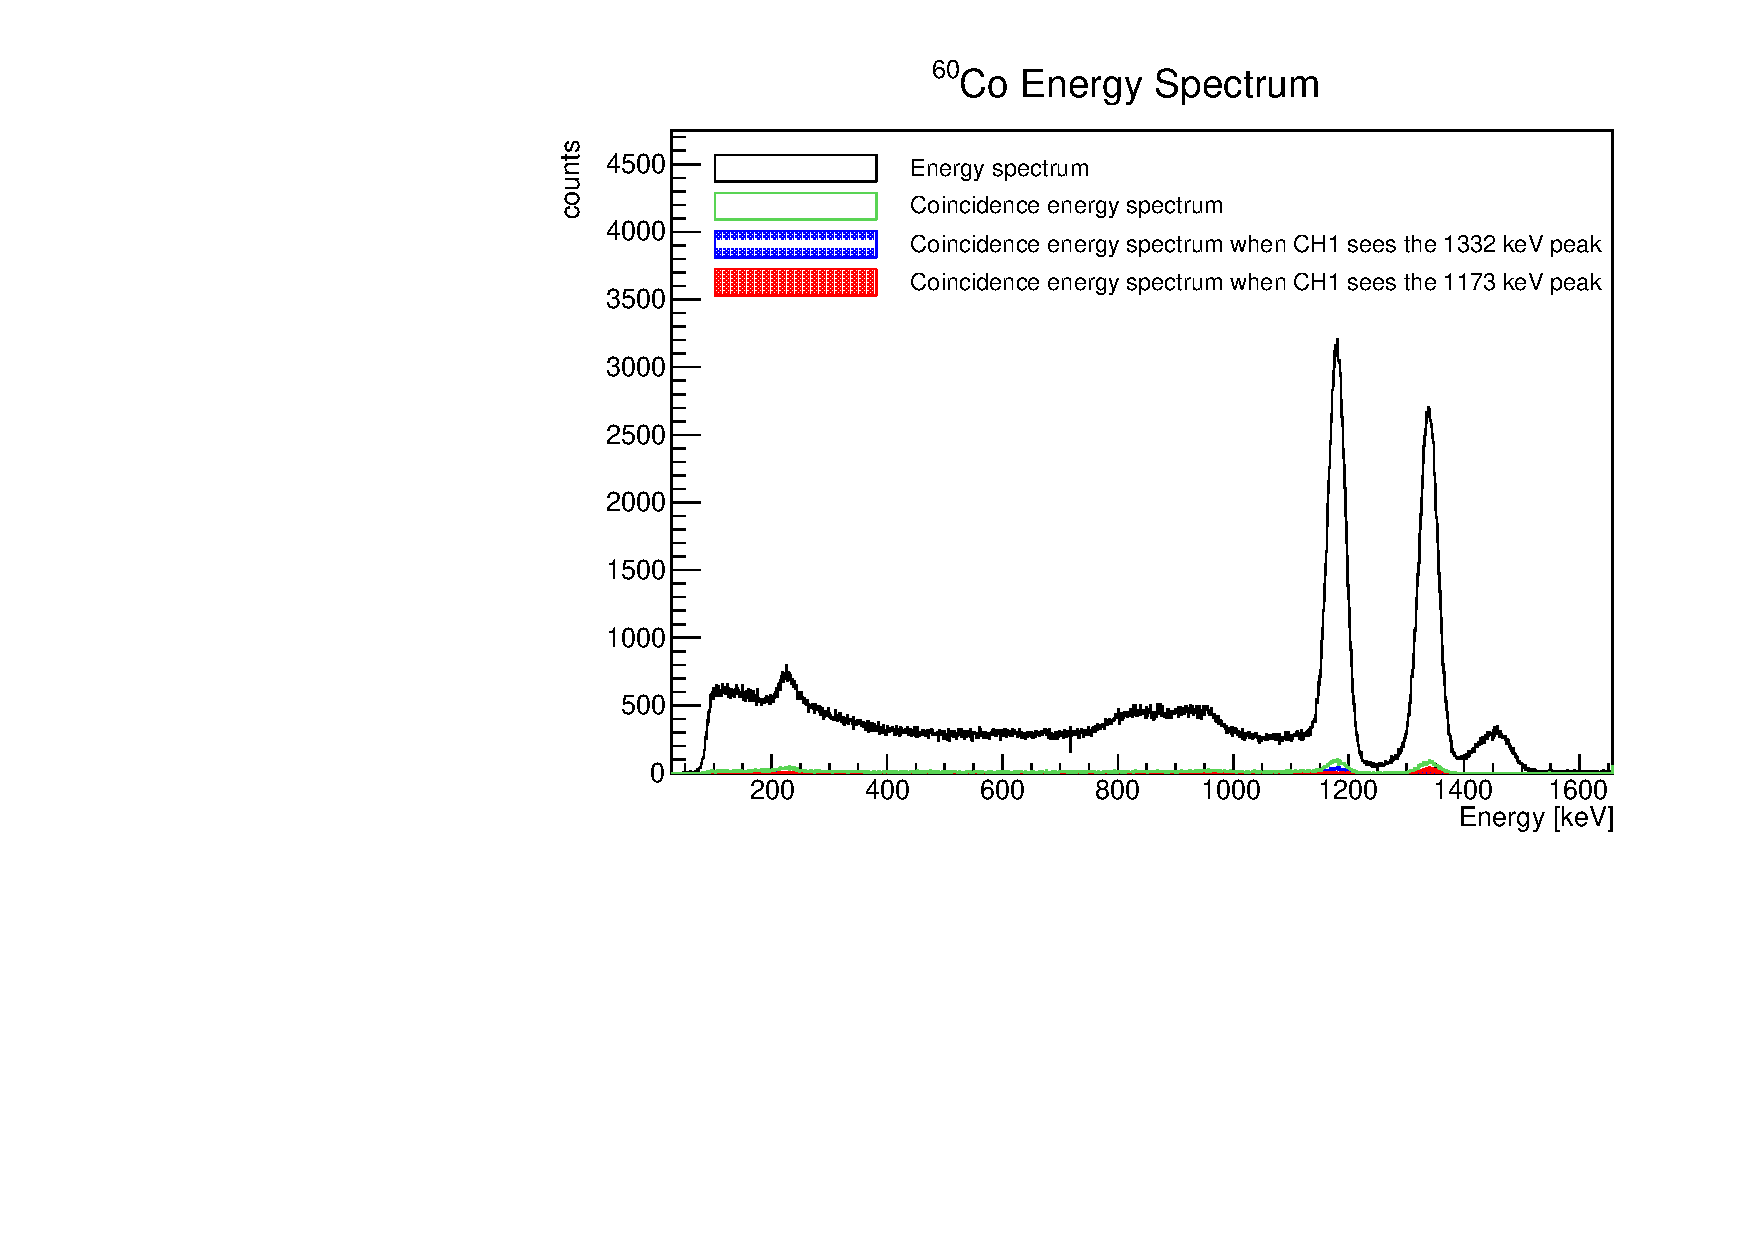
\includegraphics[width=0.9\textwidth]{Images/analysis/efficiency/Co_coinc_all.pdf} \label{fig:Co_all} }
	\end{minipage}
	\begin{minipage}[]{0.5\linewidth}
	\centering
	\subfloat[][$^{22}$Na source at 10 cm.]{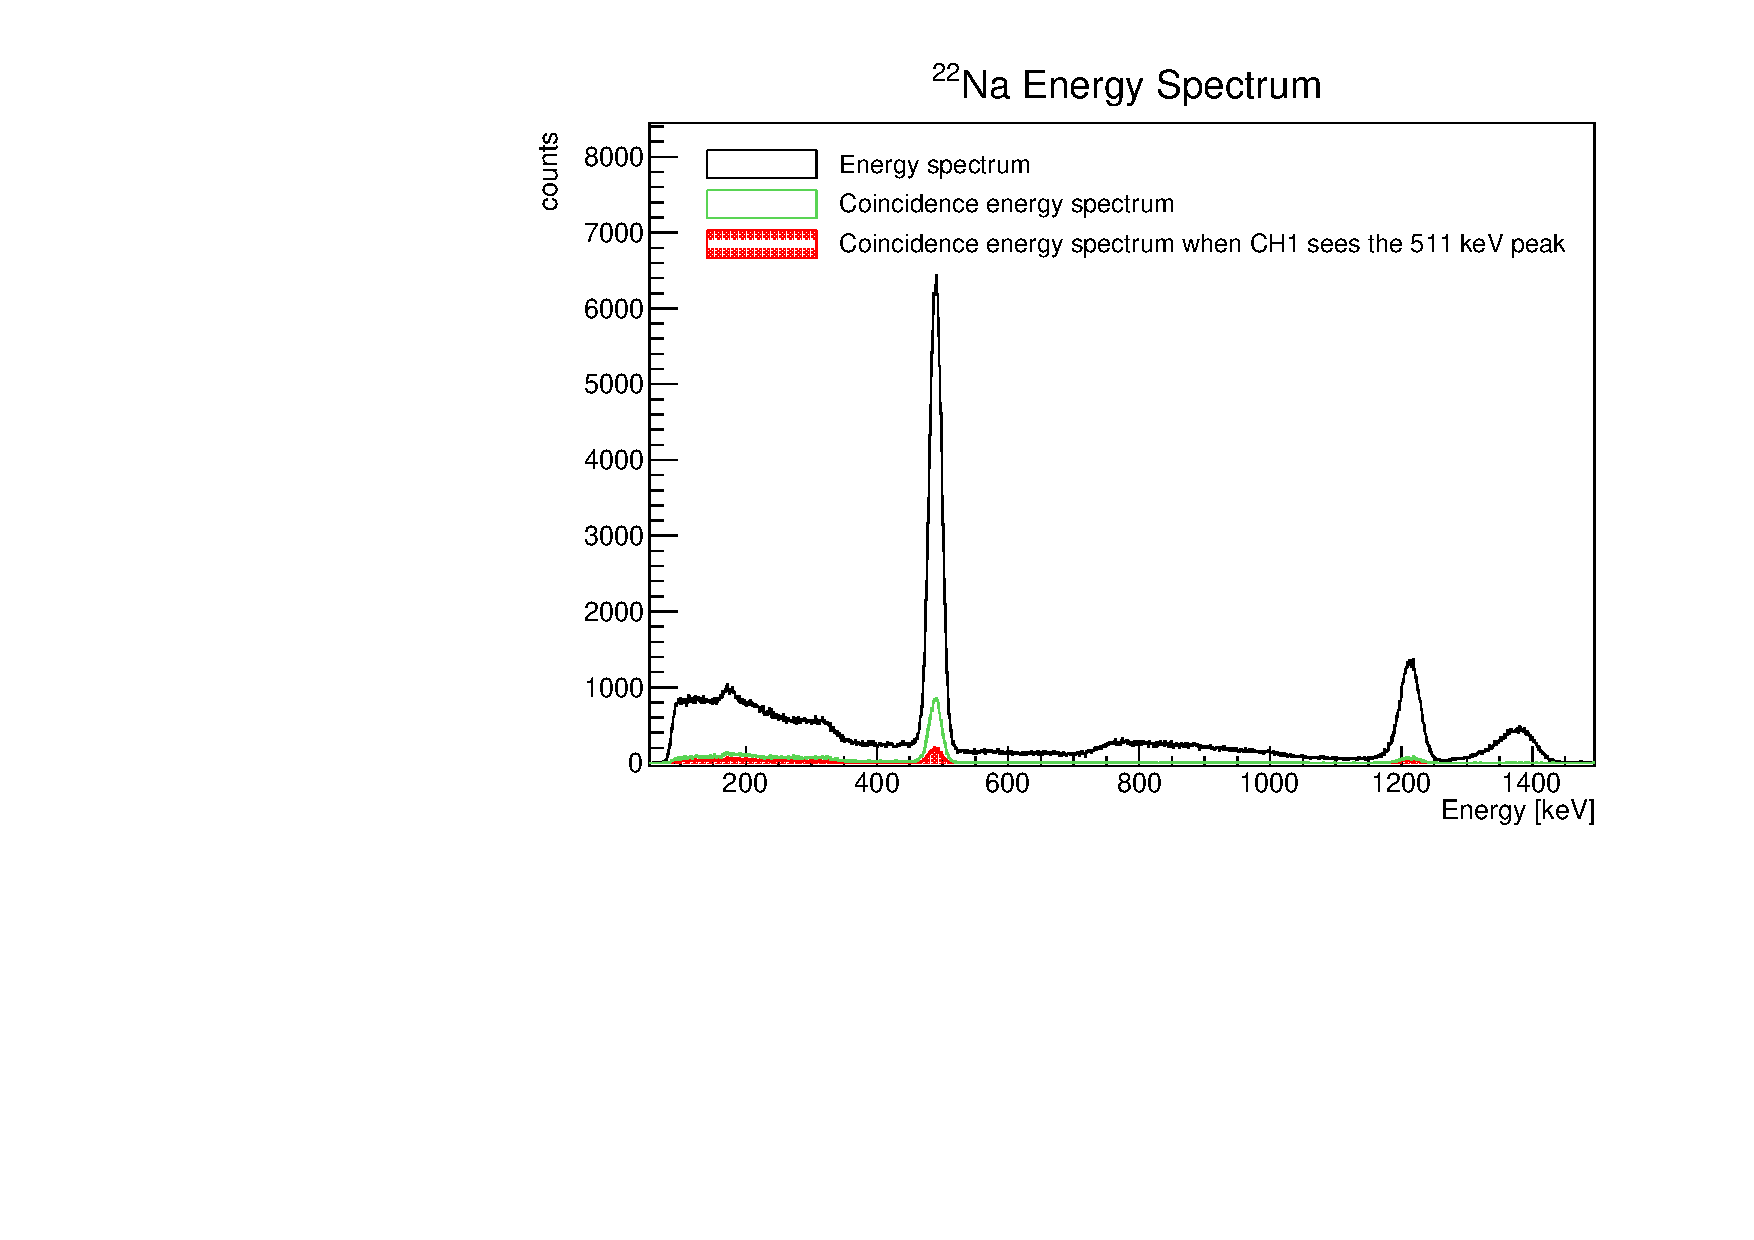
\includegraphics[width=0.9\textwidth]{Images/analysis/efficiency/Na_coinc_all.pdf}  \label{fig:Na_all} }
	\end{minipage}
	\caption{Comparison between the initial energy spectra of $^{60}$Co and $^{22}$Na, in black, the energy spectra obtained imposing coincidence between the two detectors in green, and the spectra obtained imposing the energy condition on the other detector, in red (and blue). Both spectra regard detector 0.}
    \label{fig:coinc_spectra_all}
	\end{figure}

\begin{figure}[H]
	\begin{minipage}[c]{0.5\linewidth}
	\subfloat[][$^{60}$Co source at 10 cm.]{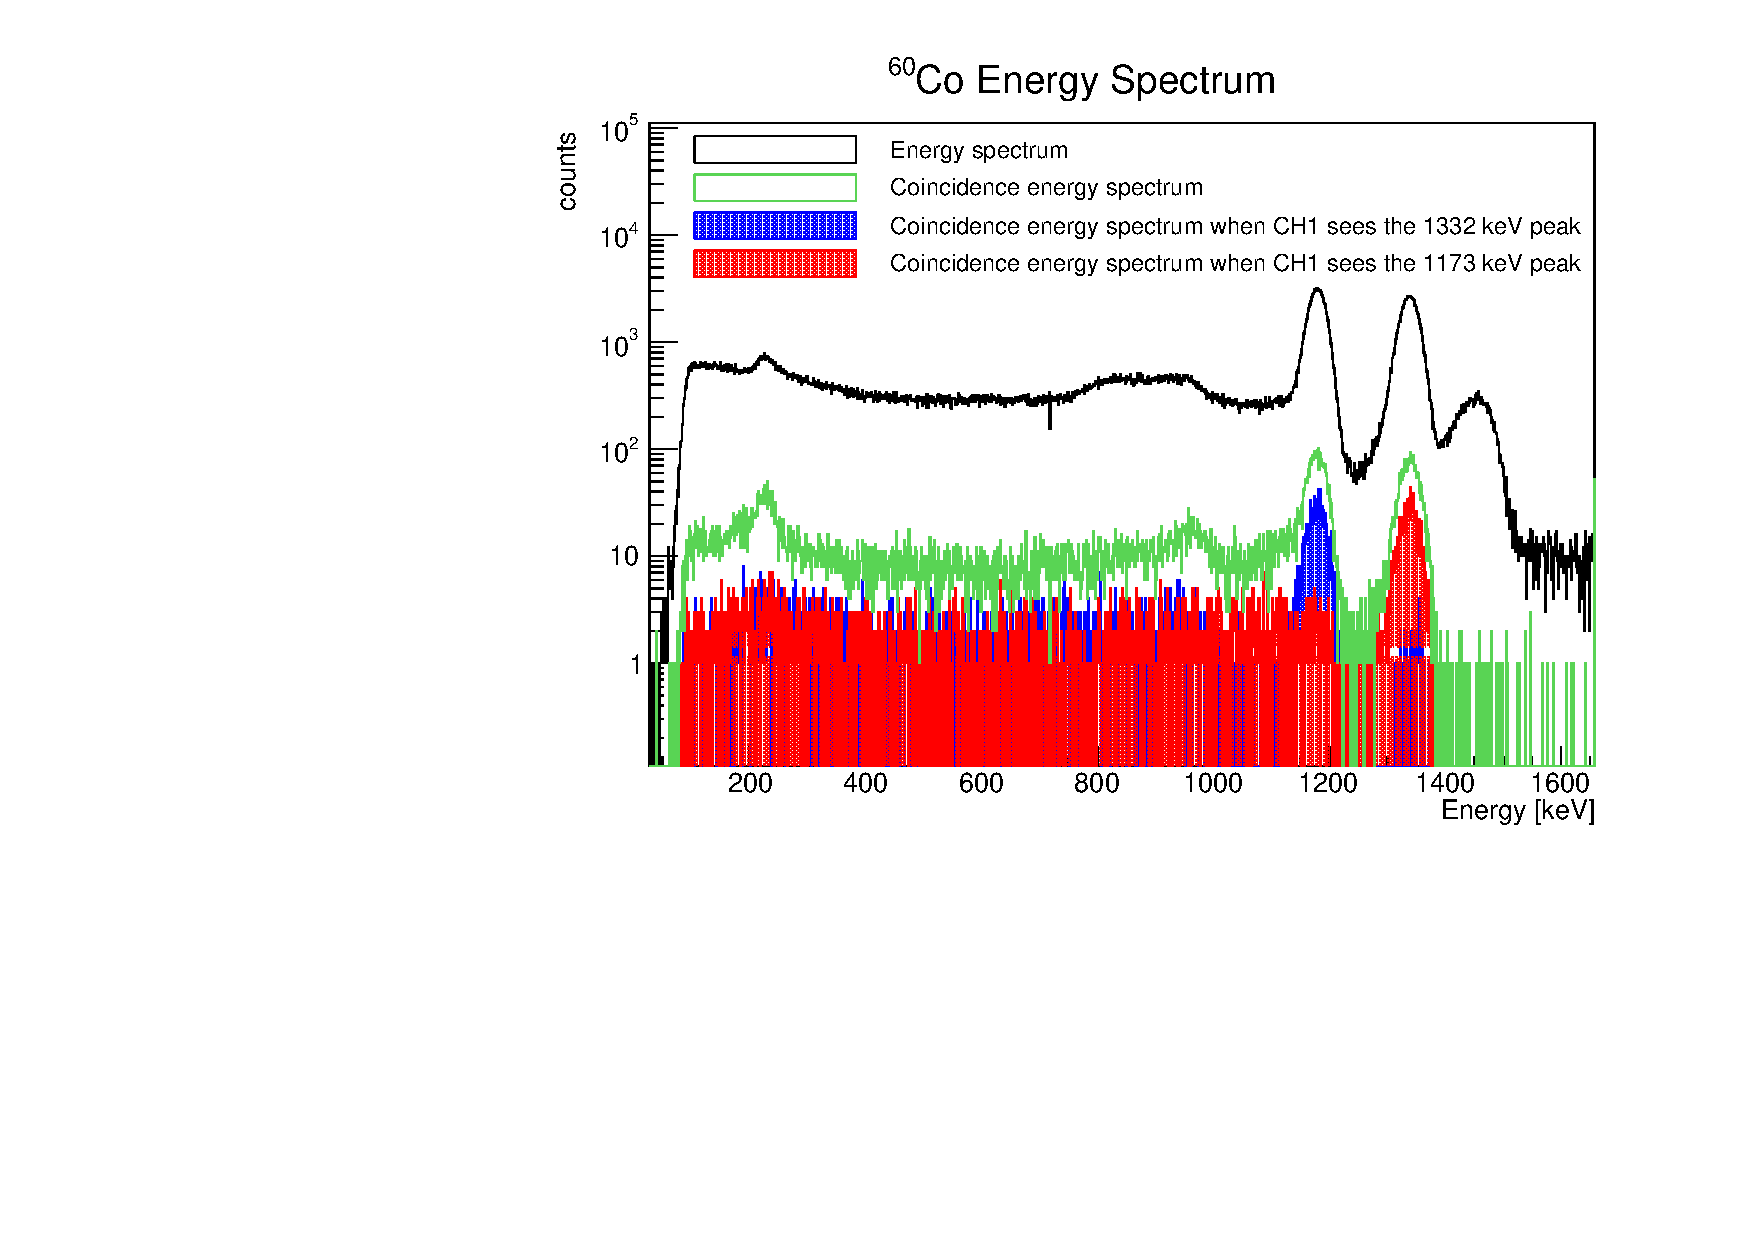
\includegraphics[width=0.9\textwidth]{Images/analysis/efficiency/Co_coinc_all_log.pdf} \label{fig:Co_all_log} }
	\end{minipage}
	\begin{minipage}[]{0.5\linewidth}
	\centering
	\subfloat[][$^{22}$Na source at 10 cm.]{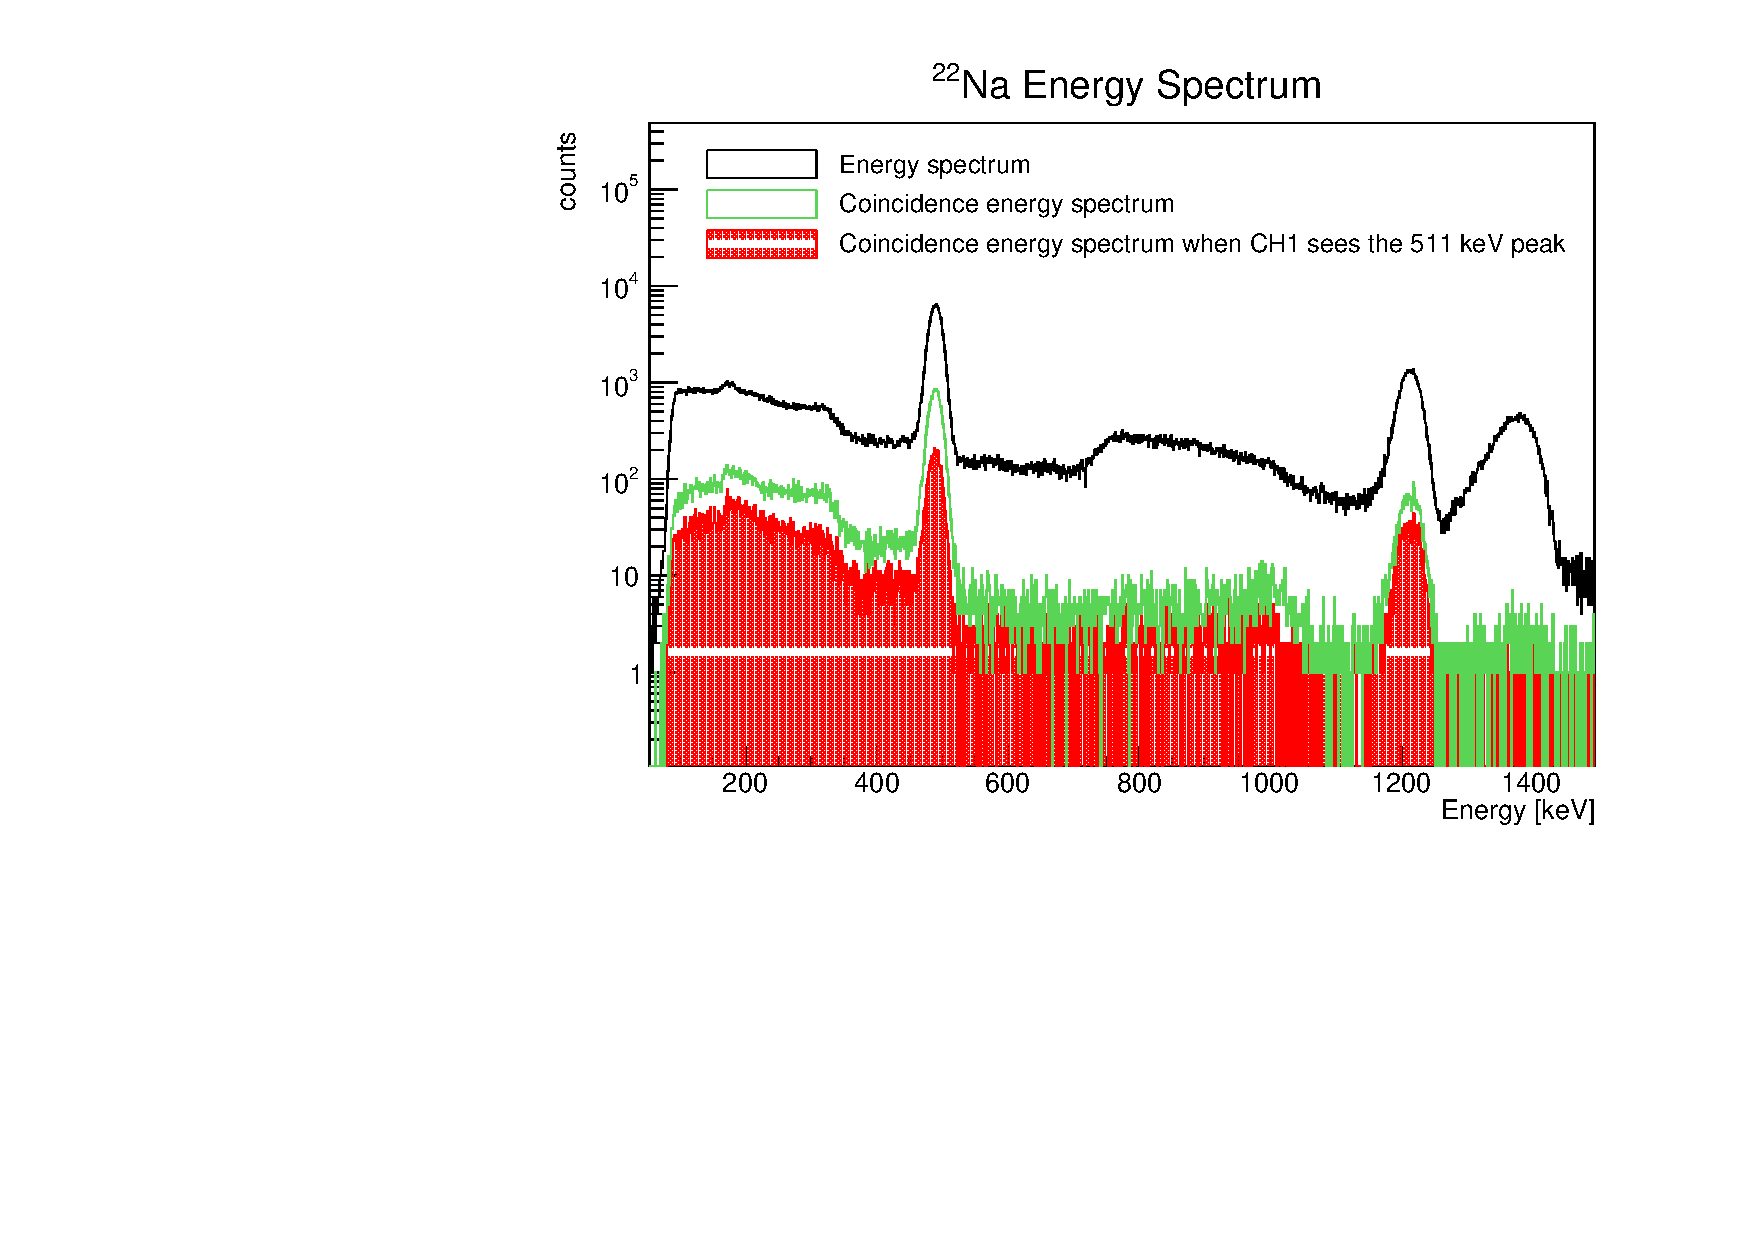
\includegraphics[width=0.9\textwidth]{Images/analysis/efficiency/Na_coinc_all_log.pdf}  \label{fig:Na_all_} }
	\end{minipage}
	\caption{Comparison between the initial energy spectra of $^{60}$Co and $^{22}$Na, in black, the energy spectra obtained imposing coincidence between the two detectors in green, and the spectra obtained imposing the energy condition on the other detector, in red (and blue). Both spectra regard detector 0.}
    \label{fig:coinc_spectra_all_log}
	\end{figure}

\begin{table}[h]
    \begin{subtable}
        \centering
        \begin{tabular}{|c|c|c|c|}
        \hline
        & E [keV]  & eff [\%] &$\sigma_{eff}$ [\%]  \\
        \hline
        $^{22}$Na at 10 cm & 511 & 2.56 & 0.08 \\
        \hline
        \multirow{2}{*}{$^{60}$Co at 10 cm}&1173 &0.92 & 0.03 \\ 
        &1332 &0.76 & 0.03 \\
        \hline
        $^{22}$Na at 15 cm & 511 & 2.47 & 0.08 \\
        \hline
        \multirow{2}{*}{$^{60}$Co at 15 cm}&1173 &0.50 & 0.02 \\ 
        &1332 &0.42 & 0.02 \\
        \hline
        $^{22}$Na at 20 cm & 511 & 2.48 & 0.08 \\
        \hline
        \multirow{2}{*}{$^{60}$Co at 20 cm}&1173 &0.24 & 0.02 \\
        &1332 &0.24& 0.02 \\
        \hline
        \end{tabular}
    \end{subtable}
    \qquad
    \qquad
    \qquad
    \begin{subtable}
        \centering
        \begin{tabular}{|c|c|c|c|}
        \hline
        & E [keV]  & eff [\%] &$\sigma_{eff}$ [\%]  \\
        \hline
        $^{22}$Na at 10 cm & 511 & 2.52 & 0.08 \\
        \hline
        \multirow{2}{*}{$^{60}$Co at 10 cm}&1173 &0.97 &0.03 \\ 
        &1332 &0.83 & 0.03 \\
        \hline
        $^{22}$Na at 15 cm & 511 & 2.47 & 0.08 \\
        \hline
        \multirow{2}{*}{$^{60}$Co at 15 cm}&1173 &0.53 & 0.02 \\ 
        &1332 &0.47 & 0.02 \\
        \hline
        $^{22}$Na at 20 cm & 511 & 2.51 & 0.08 \\
        \hline
        \multirow{2}{*}{$^{60}$Co at 20 cm}&1173 &0.28 & 0.02 \\
        &1332 &0.21 & 0.01 \\
        \hline
        \end{tabular}
     \end{subtable}
     \caption{Values of efficiency for the $^{60}$Co source at different distances, imposing the coincidence between the detectors and the condition that in the other we see the other peak, for detector 0 and 1 respectively}
     \label{tab:eff_coin_en}
\end{table}

\begin{figure}[H]
    \centering
    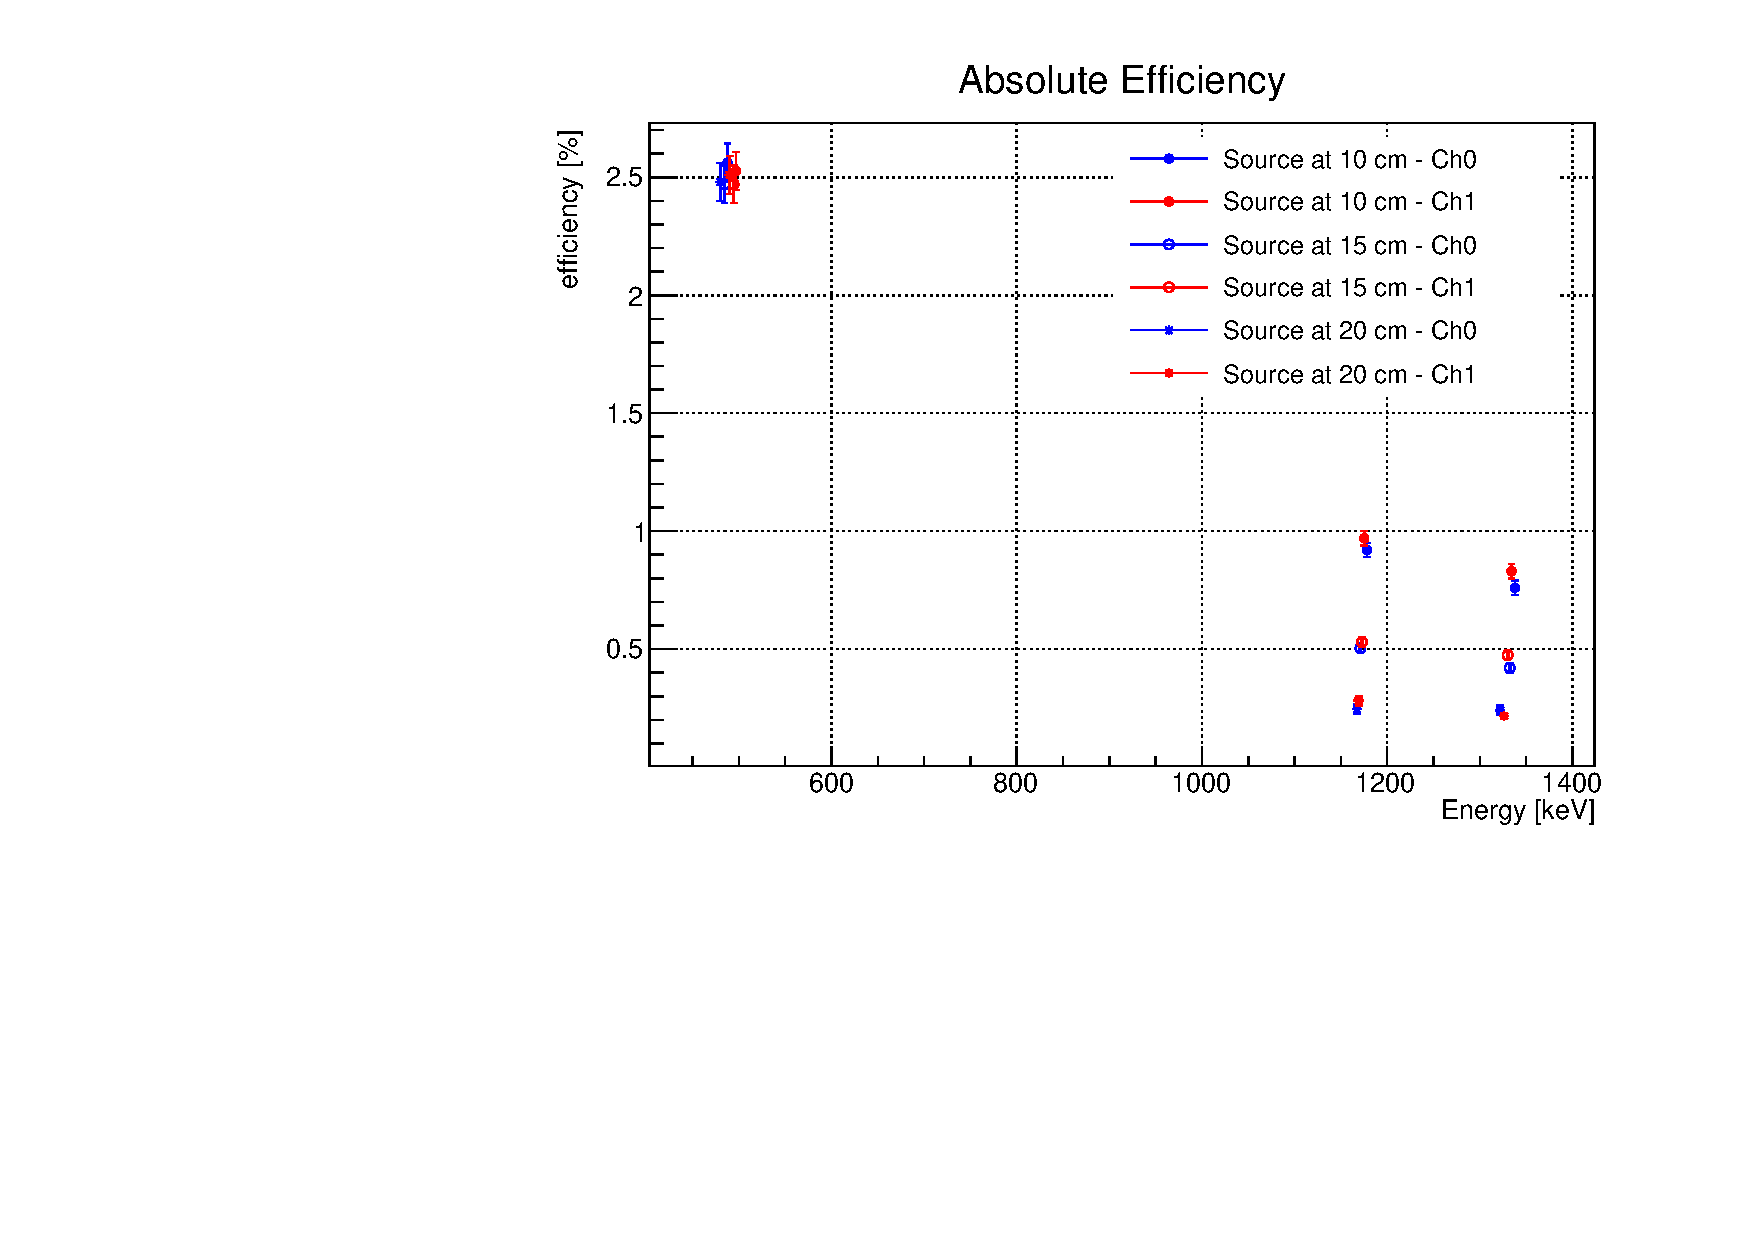
\includegraphics[scale=0.5]{Images/analysis/efficiency/Eff_all.pdf}
    \caption{Efficiency of the detectors, imposing coincidences, energy condition and considering summing up as in \ref{eq:eta}, with detector 0 in blue and detector 1 in red, for all the distances.}
    \label{fig:eff_all}
\end{figure}

\begin{figure}[H]
	\begin{minipage}[c]{0.35\linewidth}
    \centering
	\subfloat[][Sources at 10 cm.]{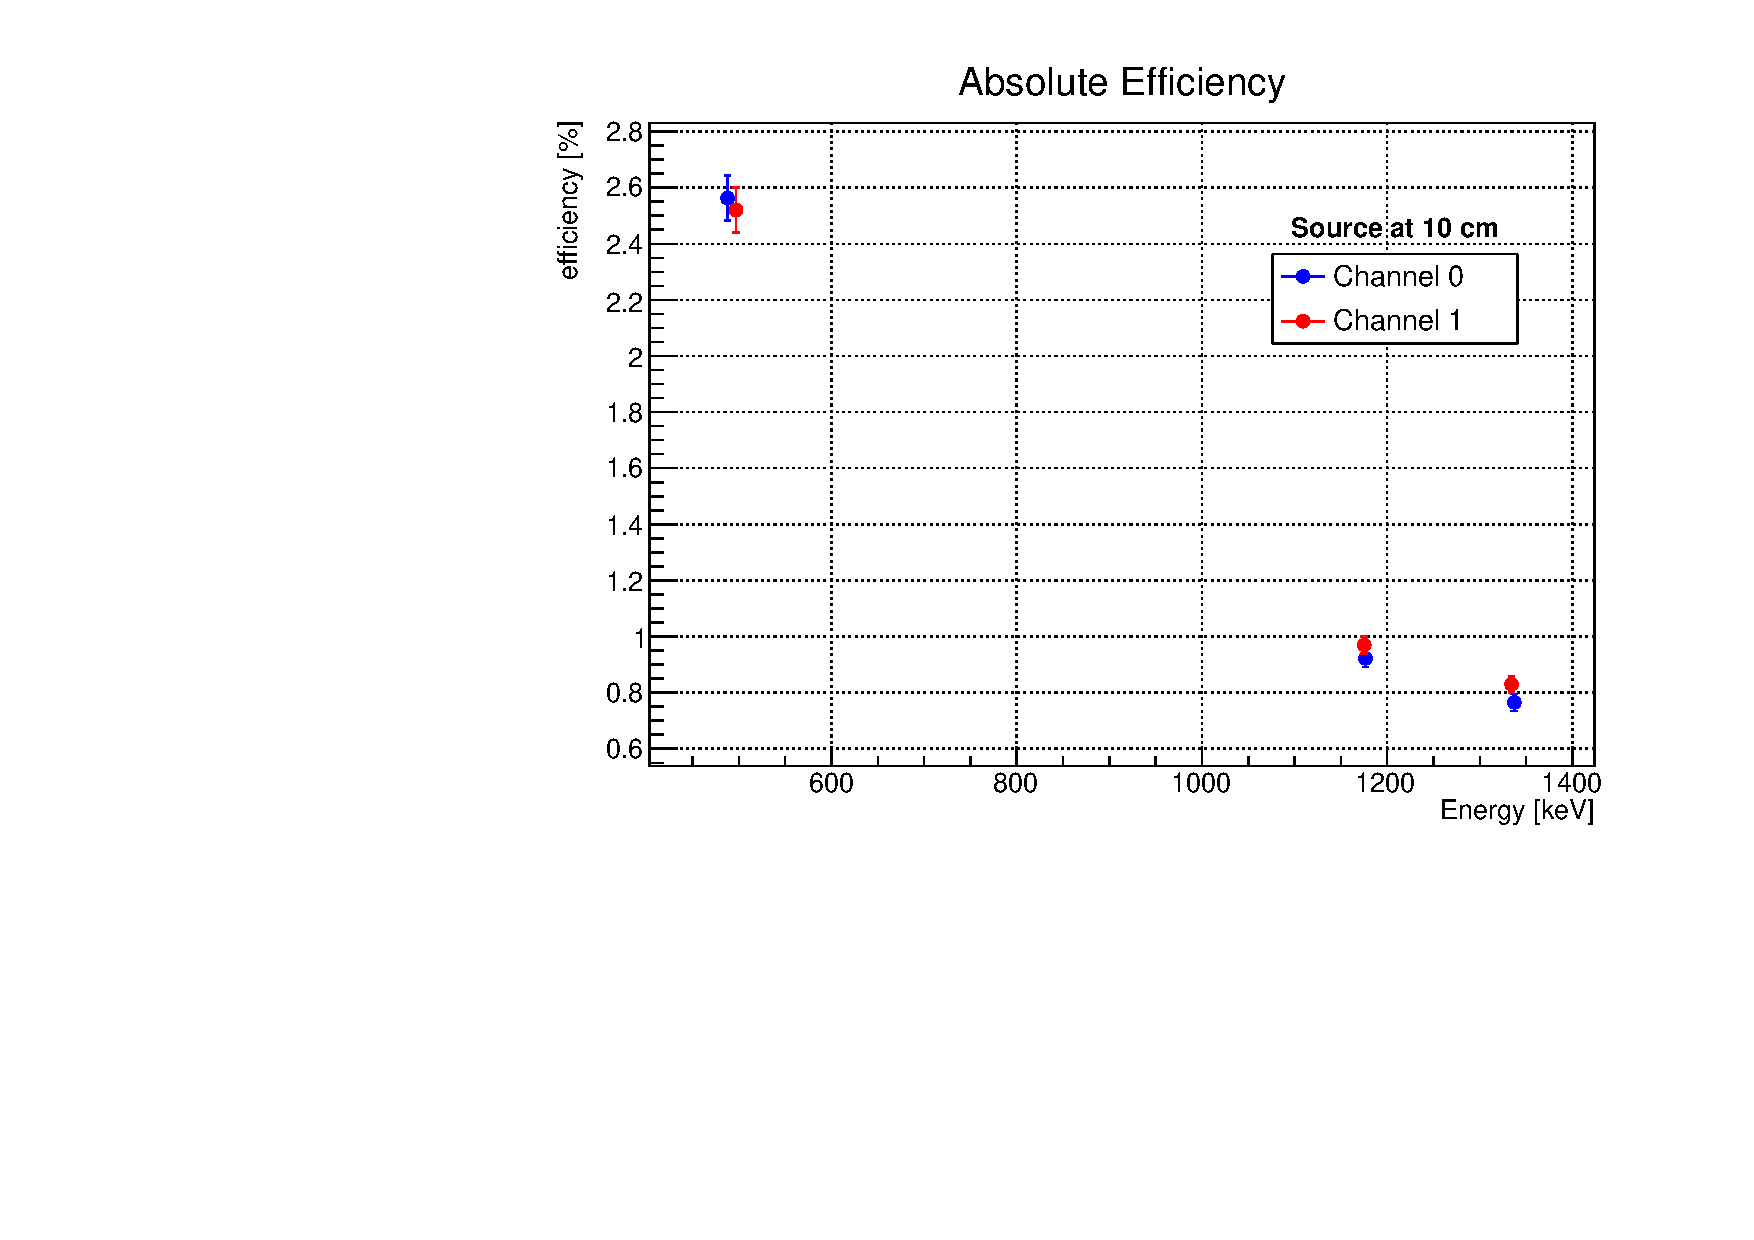
\includegraphics[width=0.95\textwidth]{Images/analysis/efficiency/eff_all_10.pdf}\label{fig:all_10} }
	\end{minipage}
	\begin{minipage}[]{0.35\linewidth}
	\centering
	\subfloat[][Sources at 15 cm.]{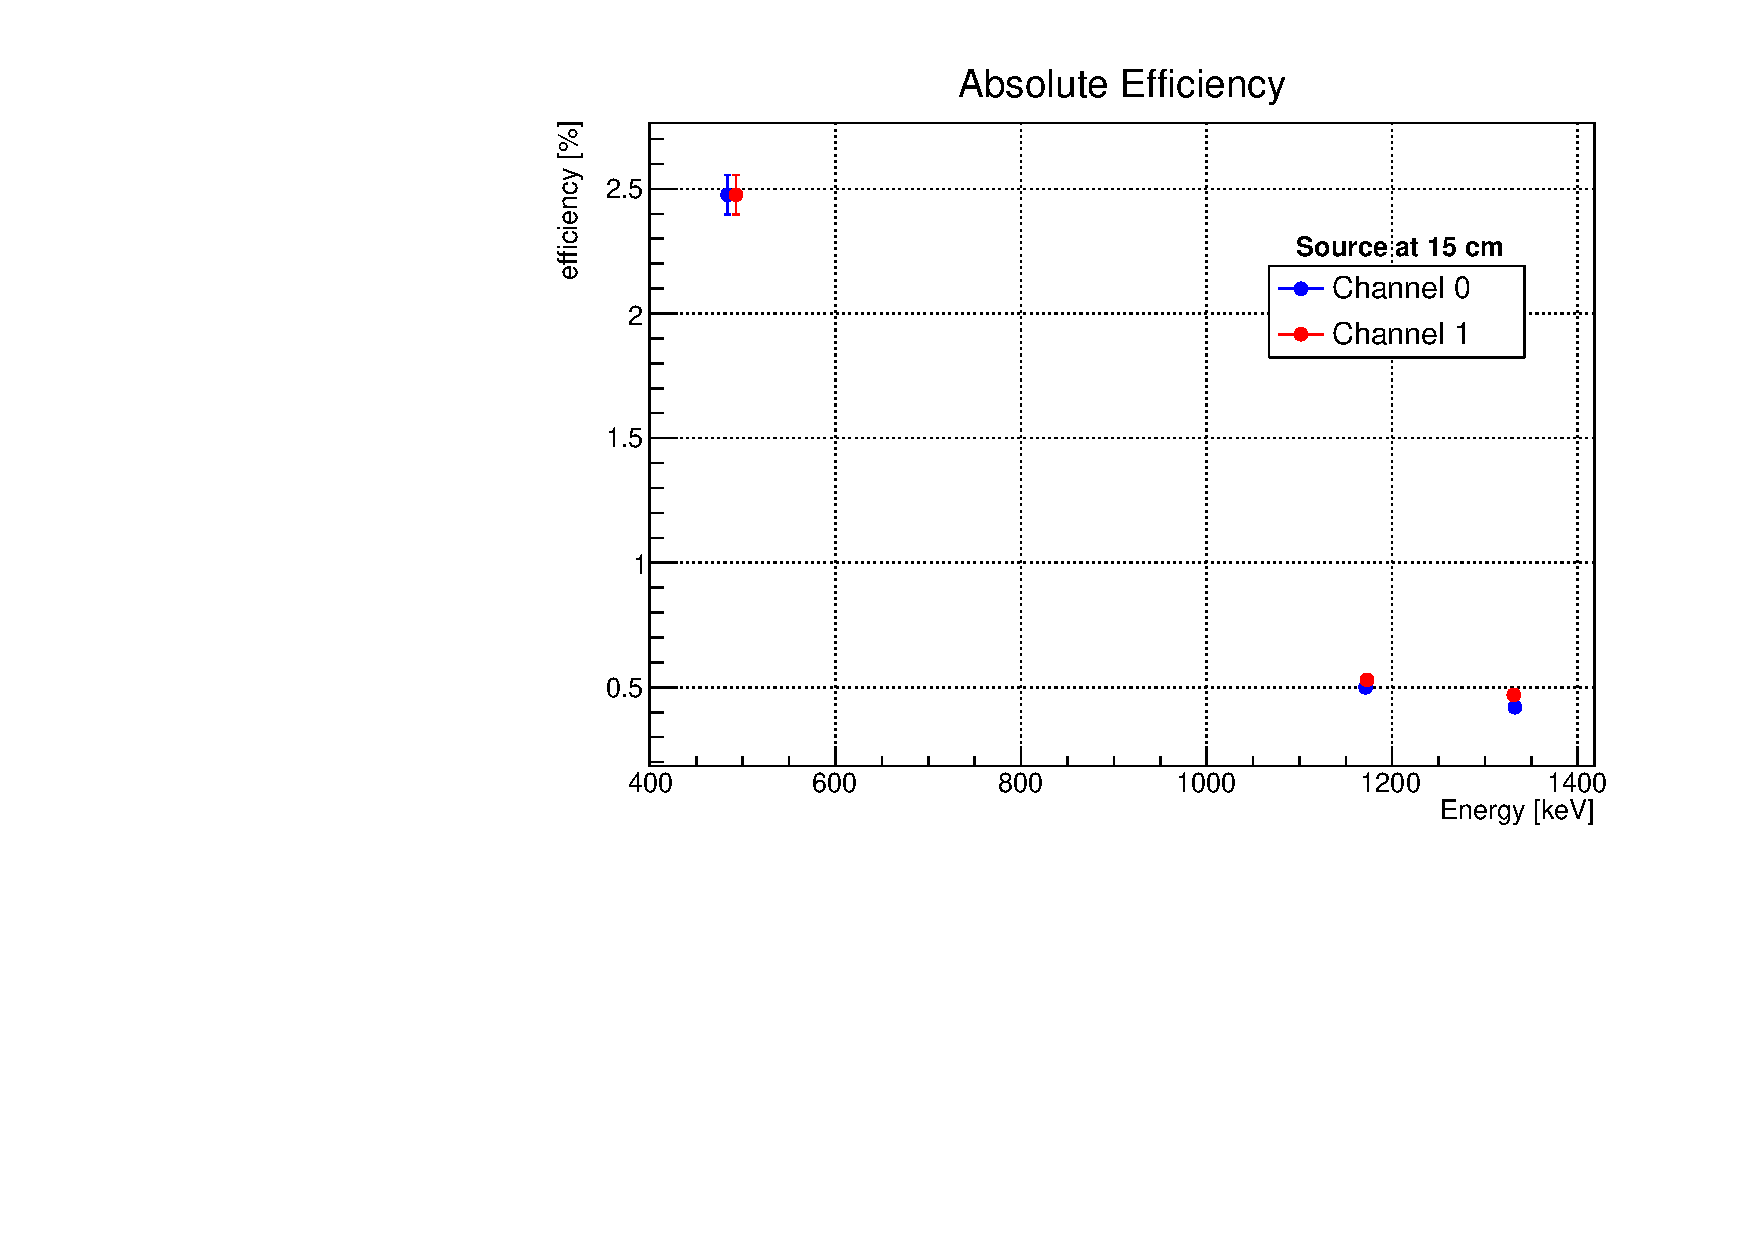
\includegraphics[width=0.95\textwidth]{Images/analysis/efficiency/eff_all_15.pdf}  \label{fig:all_15} }
	\end{minipage}
    \begin{minipage}[c]{0.35\linewidth}
    \centering
	\subfloat[][Source at 20 cm]{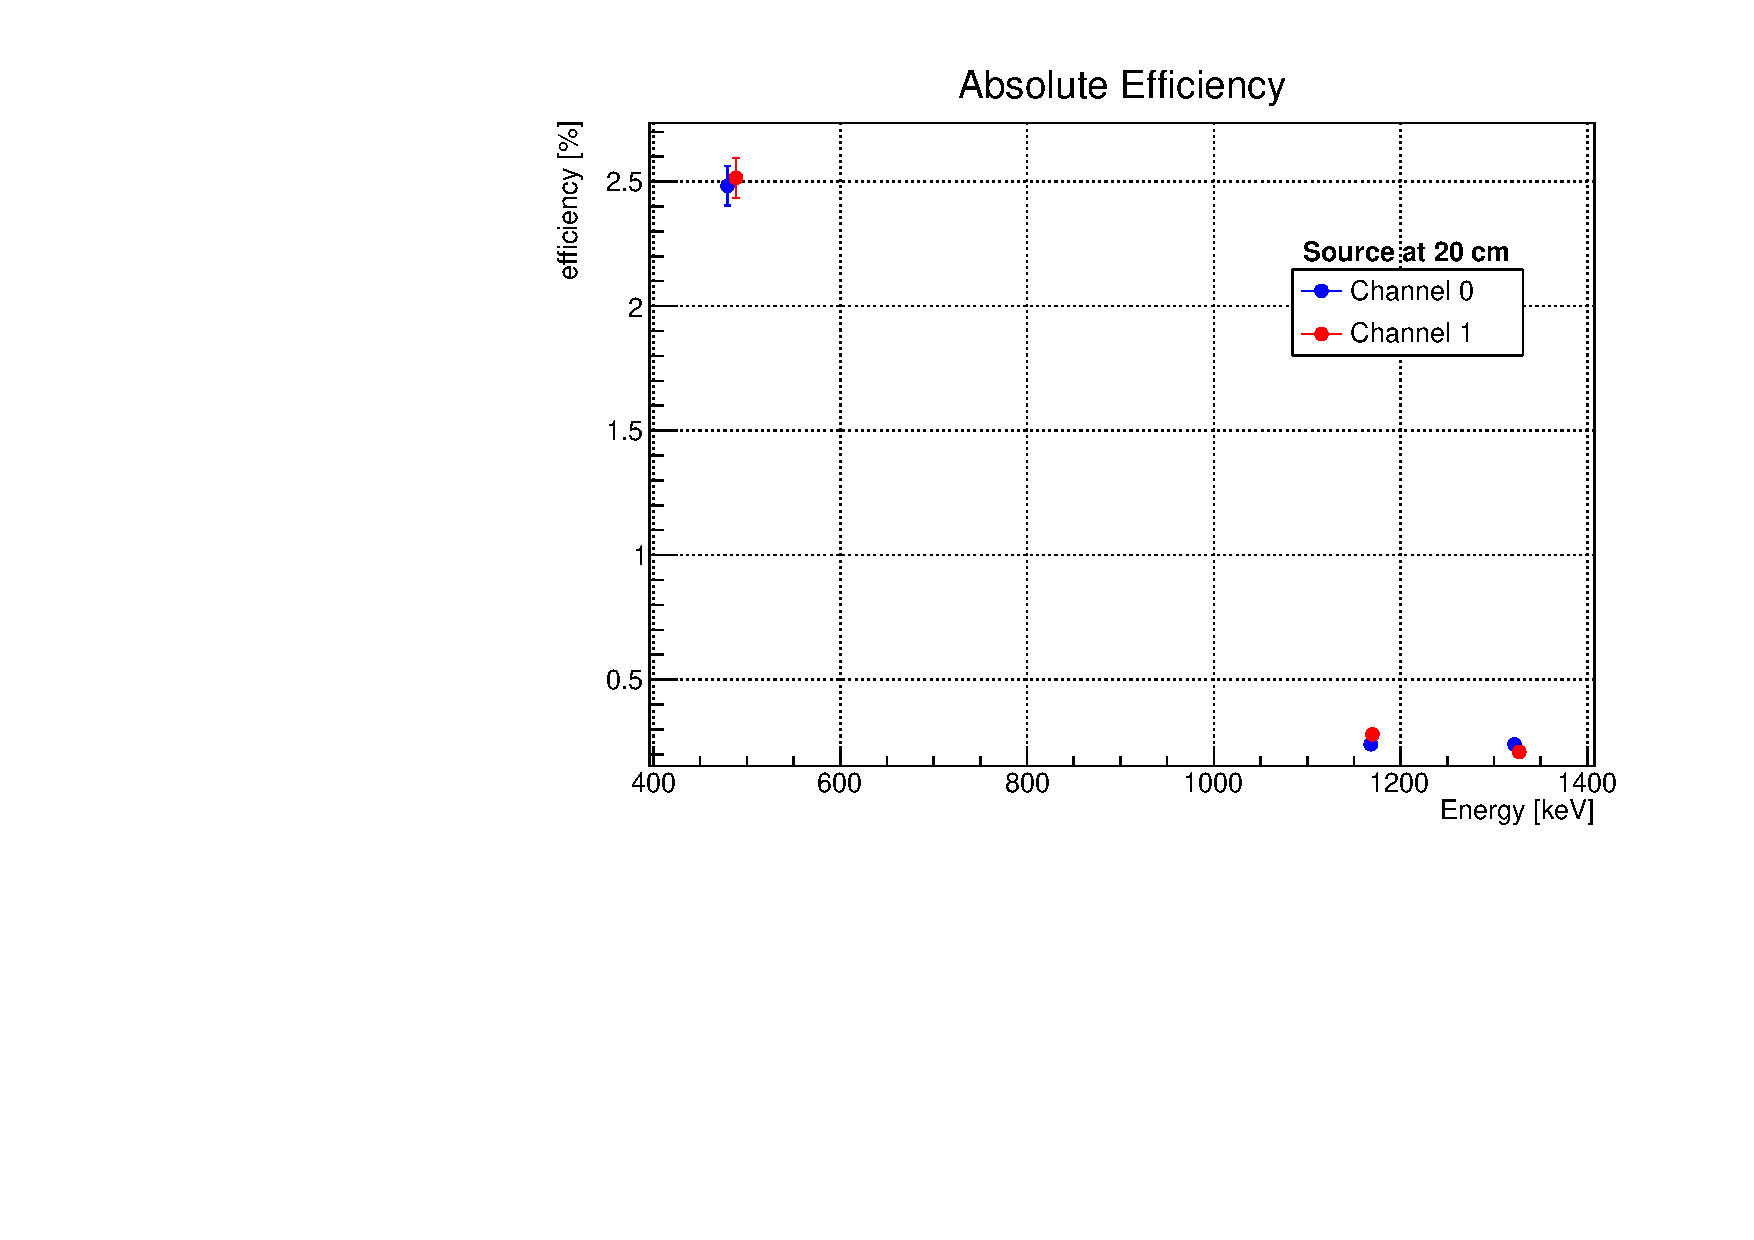
\includegraphics[width=0.95\textwidth]{Images/analysis/efficiency/eff_all_20.pdf}\label{fig:all_20}} 
	\end{minipage}
	\caption{Efficiency of the detectors, imposing coincidences, energy condition and considering summing up as in \ref{eq:eta}, with detector 0 in blue and detector 1 in red, at each different distances for each plot.}
    \label{fig:eff_all3}
	\end{figure}

     




